\documentclass[compress]{beamer}
\usepackage{ifthen,verbatim,ulem}

\newcommand{\isnote}{}
\xdefinecolor{lightyellow}{rgb}{1.,1.,0.25}
\xdefinecolor{darkblue}{rgb}{0.1,0.1,0.7}

%% Uncomment this to get annotations
%% \def\notes{\addtocounter{page}{-1}
%%            \renewcommand{\isnote}{*}
%% 	   \beamertemplateshadingbackground{lightyellow}{white}
%%            \begin{frame}
%%            \frametitle{Notes for the previous page (page \insertpagenumber)}
%%            \itemize}
%% \def\endnotes{\enditemize
%% 	      \end{frame}
%%               \beamertemplateshadingbackground{white}{white}
%%               \renewcommand{\isnote}{}}

%% Uncomment this to not get annotations
\def\notes{\comment}
\def\endnotes{\endcomment}

\setbeamertemplate{navigation symbols}{}
\setbeamertemplate{headline}{\mbox{ } \hfill
\begin{minipage}{5.5 cm}
\vspace{-0.75 cm} \small
\end{minipage} \hfill
\begin{minipage}{4.5 cm}
\vspace{-0.75 cm} \small
\begin{flushright}
\ifthenelse{\equal{\insertpagenumber}{1}}{}{Jim Pivarski \hspace{0.2 cm} \insertpagenumber\isnote/\pageref{numpages}}
\end{flushright}
\end{minipage}\mbox{\hspace{0.2 cm}}\includegraphics[height=1 cm]{../cmslogo} \hspace{0.1 cm} \includegraphics[height=1 cm]{../tamulogo} \hspace{0.01 cm} \vspace{-1.05 cm}}

\begin{document}
\begin{frame}
\vfill
\begin{center}
\textcolor{darkblue}{\Large Alignment of the DT chambers \\ \vspace{0.2 cm} with a HIP-based algorithm}

\vfill
\begin{columns}
\column{0.3\linewidth}
\begin{center}
\large
\textcolor{darkblue}{Jim Pivarski}

\vspace{0.2 cm}
Alexei Safonov
\end{center}
\end{columns}

\begin{columns}
\column{0.3\linewidth}
\begin{center}
\scriptsize
{\it Texas A\&M University}
\end{center}
\end{columns}

\vfill
29 January, 2009

\end{center}
\end{frame}

%% \begin{notes}
%% \item This is the annotated version of my talk.
%% \item If you want the version that I am presenting, download the one
%% labeled ``slides'' on Indico (or just ignore these yellow pages).
%% \item The annotated version is provided for extra detail and a written
%% record of comments that I intend to make orally.
%% \item Yellow notes refer to the content on the {\it previous} page.
%% \item All other slides are identical for the two versions.
%% \end{notes}

\small

\begin{frame}
\frametitle{Overview}
\framesubtitle{How does DT alignment fit into our plans?}

\vfill
\mbox{\hspace{-1 cm}\begin{minipage}{1.1\linewidth}
\begin{description}
\item[\textcolor{black}{Goal:}] align the whole muon system with a consistent HIP-based procedure in the same coordinate system used by the tracker
\end{description}
\end{minipage}}

\vfill
\begin{itemize}\setlength{\itemsep}{0.25 cm}
\item Limitation of cosmic rays: distribution doesn't illuminate sides
  of the detector well, and statistics for tracks that link the
  tracker and the muon endcap are especially poor

\item CRAFT plan:
\begin{enumerate}
\item align well-illuminated DT chambers relative to the tracker with globalMuons
\item align remaining DT chambers relative to aligned DT chambers with standAloneMuons
\item align CSCs relative to aligned barrel with standAloneMuons
\end{enumerate}

\item Step 1 is complete, with supporting evidence
  demonstrating that this is a true alignment, not simply a
  minimization of residuals

\item We are ready to submit these constants for CRAFT re-processing
\end{itemize}

%% \hspace{-0.83 cm} \textcolor{darkblue}{\Large Outline2}
\end{frame}

\begin{frame}
\frametitle{Outline for this talk}
\begin{itemize}\setlength{\itemsep}{0.25 cm}
\item Basic description of the procedure
\item Detailed study of residuals, controlling for systematic effects
\begin{itemize}
\item effect of $\vec{B}$-field mismodelling
\item effect of multiple scattering
\item effect of biases in the track source
\item effect of non-uniform illumination of the chambers
\end{itemize}

\item Validation plots
\begin{itemize}
\item comparison with old constants (CRAFT\_ALL\_V4) and MillePede Group's constants
\end{itemize}

\item Conclusion: summary of proposed HIP constants

\item Epilogue: discovered a chamber description error; \mbox{early investigations\hspace{-1 cm}}
\end{itemize}
\end{frame}

\begin{frame}
\frametitle{HIP-based procedure}

\begin{columns}
\column{0.35\linewidth}
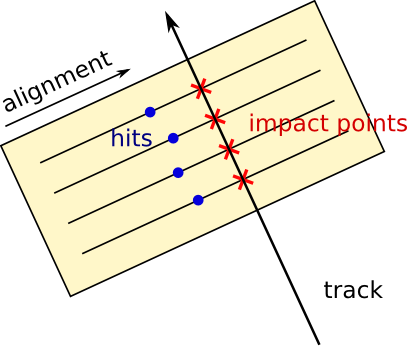
\includegraphics[width=\linewidth]{hip_explanation.png}

\column{0.65\linewidth}

\textcolor{darkblue}{HIP algorithm: ``Hits and Impact Points''}
\begin{itemize}
\item Using a track as reference, alignment correction is the peak of the residuals distribution

\item Our $\mbox{residual} \equiv \left(\mbox{impact point}\right) - \left(\mbox{hit}\right)$

\end{itemize}
\end{columns}

\vspace{0.2 cm}
Implementation is not exactly the same as that in the tracker

\vspace{0.1 cm}
\textcolor{darkblue}{Important differences:}
\begin{itemize}
\item Muon hits excluded from refitted tracks: tracker is \mbox{external reference\hspace{-1 cm}}
\begin{itemize}
\item breaks the circularity between fitting tracks and \mbox{aligning chambers\hspace{-1 cm}}
\item no need to iterate: convergence in one step
\end{itemize}
\item Only hits within a chamber on one track are averaged with weights
\begin{itemize}
\item handles statistics of correlated hits properly
\end{itemize}
\item Muon chambers are much bigger than silicon wafers: study
  residuals as a function of position throughout each chamber
\end{itemize}
\end{frame}

\begin{frame}
\frametitle{Effect of $\vec{B}$-field mismodelling}

\begin{itemize}
\item Magnetic field is known to be mismodelled at the level of 30\%
\item Track propagation is sensitive to integral of $\vec{B}$-field error along \mbox{its path\hspace{-1 cm}}
\item How can we get reliable residuals?
\end{itemize}

\begin{columns}
\column{0.6\linewidth}
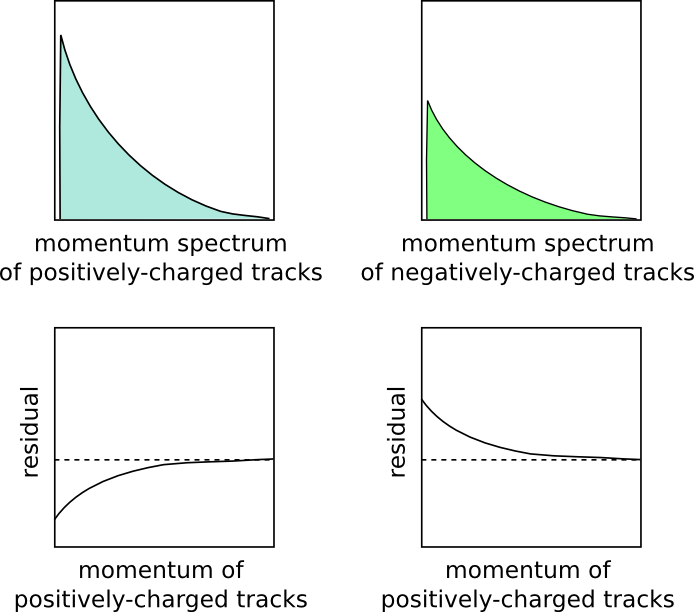
\includegraphics[width=\linewidth]{momentum_explanation.png}

\column{0.4\linewidth}
\vspace{-1 cm}
\begin{itemize}
\item Number of positively-charged and negatively-charged muons is not
  equal, but the momentum spectra are identical (fact used in charge
  ratio analysis)

\item Small deviations of reconstructed track from average muon
  trajectory is antisymmetric with charge
\end{itemize}
\end{columns}
\end{frame}

\begin{frame}
\frametitle{Effect of $\vec{B}$-field mismodelling}

\vspace{0.5 cm}
\begin{columns}
\column{0.6\linewidth}
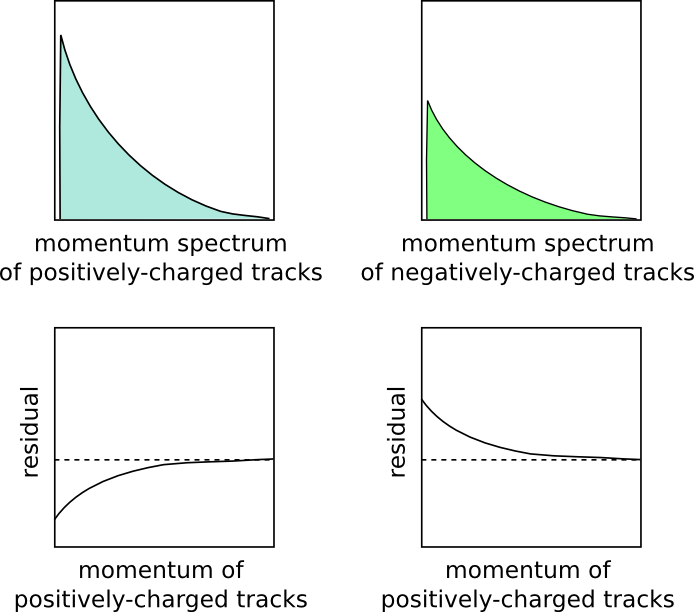
\includegraphics[width=\linewidth]{momentum_explanation.png}

\column{0.4\linewidth}
\vspace{-1 cm}
\begin{itemize}
\item Measure residuals peak in two bins, one for each charge
\item Non-weighted average is insensitive to $\vec{B}$-field errors

$\displaystyle \mbox{alignment} = \frac{R_+ + R_-}{2}$

\item Difference is maximally sensitive

$\displaystyle \mbox{error tracer} = \frac{R_+ - R_-}{2}$

\end{itemize}
\end{columns}

\begin{itemize}
\item Effectively scales up negatively-charged muon statistics such that the two curves cancel
\item \mbox{$\displaystyle \mbox{Systematic error} = \left(\mbox{error tracer}\right) \times \left(\mbox{charge mismeasurement}\right) \times \frac{0.3}{2.3}$}

\textcolor{white}{$\mbox{Systematic error}$} $\sim \left(\mbox{error tracer}\right) \times \left(\mbox{a few percent or less}\right)$

\end{itemize}
\end{frame}

\begin{frame}
\frametitle{Effect of $\vec{B}$-field mismodelling}
\begin{itemize}
\item Demonstration in station 4 (largest $\vec{B}$-field errors):
\begin{itemize}
\item despite large $(R_+ - R_-)/2$ difference (``error tracer''),

\vspace{0.2 cm}
the $(R_+ + R_-)/2$ average cleanly breaks at chamber boundaries
\end{itemize}
\end{itemize}

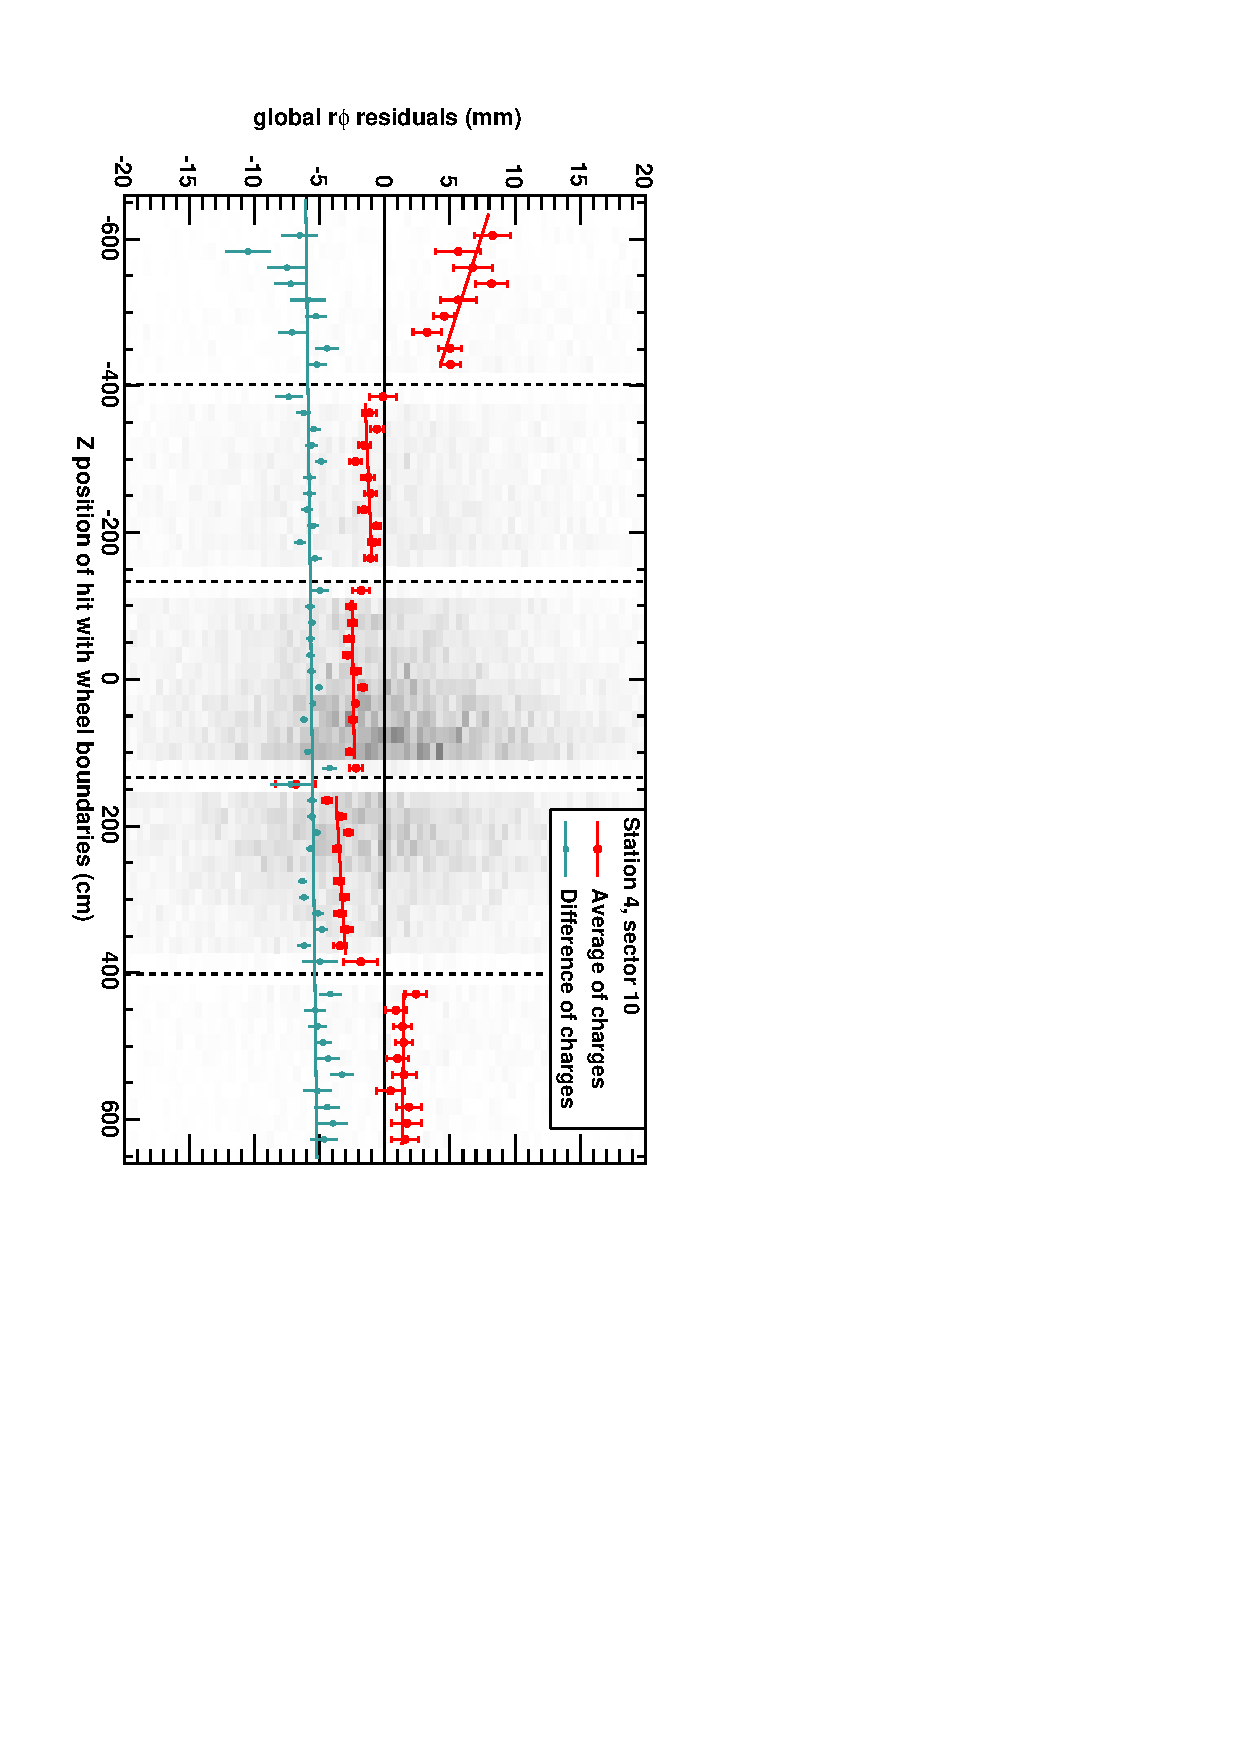
\includegraphics[height=\linewidth, angle=90]{demo_of_bfield.pdf}

\scriptsize grey background is the raw 2-D residuals distribution

linear fits are only a guide for the eye: not used in alignment!
\end{frame}

\begin{frame}
\frametitle{Effect of multiple scattering}

\begin{itemize}
\item Alignment correction is the peak of the \mbox{residuals distribution because\hspace{-1 cm}}
\begin{itemize}
\item good tracks agree about the alignment correction
\item bad tracks (which scatter) disagree in different ways
\end{itemize}
\end{itemize}

\begin{columns}
\column{0.65\linewidth}
Scattering processes follow \mbox{power-law distributions,\hspace{-1 cm}} while
  experimental resolution is Gaussian

\vspace{-0.5 cm}
\begin{multline*}
f(x) = \int_{-\infty}^\infty \frac{1}{\pi}\frac{\Gamma/2}{(x - \xi)^2 + (\Gamma/2)^2} \times \\
\frac{1}{\sqrt{2\pi} \sigma} \exp\left(\frac{-\xi^2}{2 \sigma^2}\right) \, d\xi
\end{multline*}

The peak of every subset of residuals is determined from an unbinned fit

\column{0.35\linewidth}
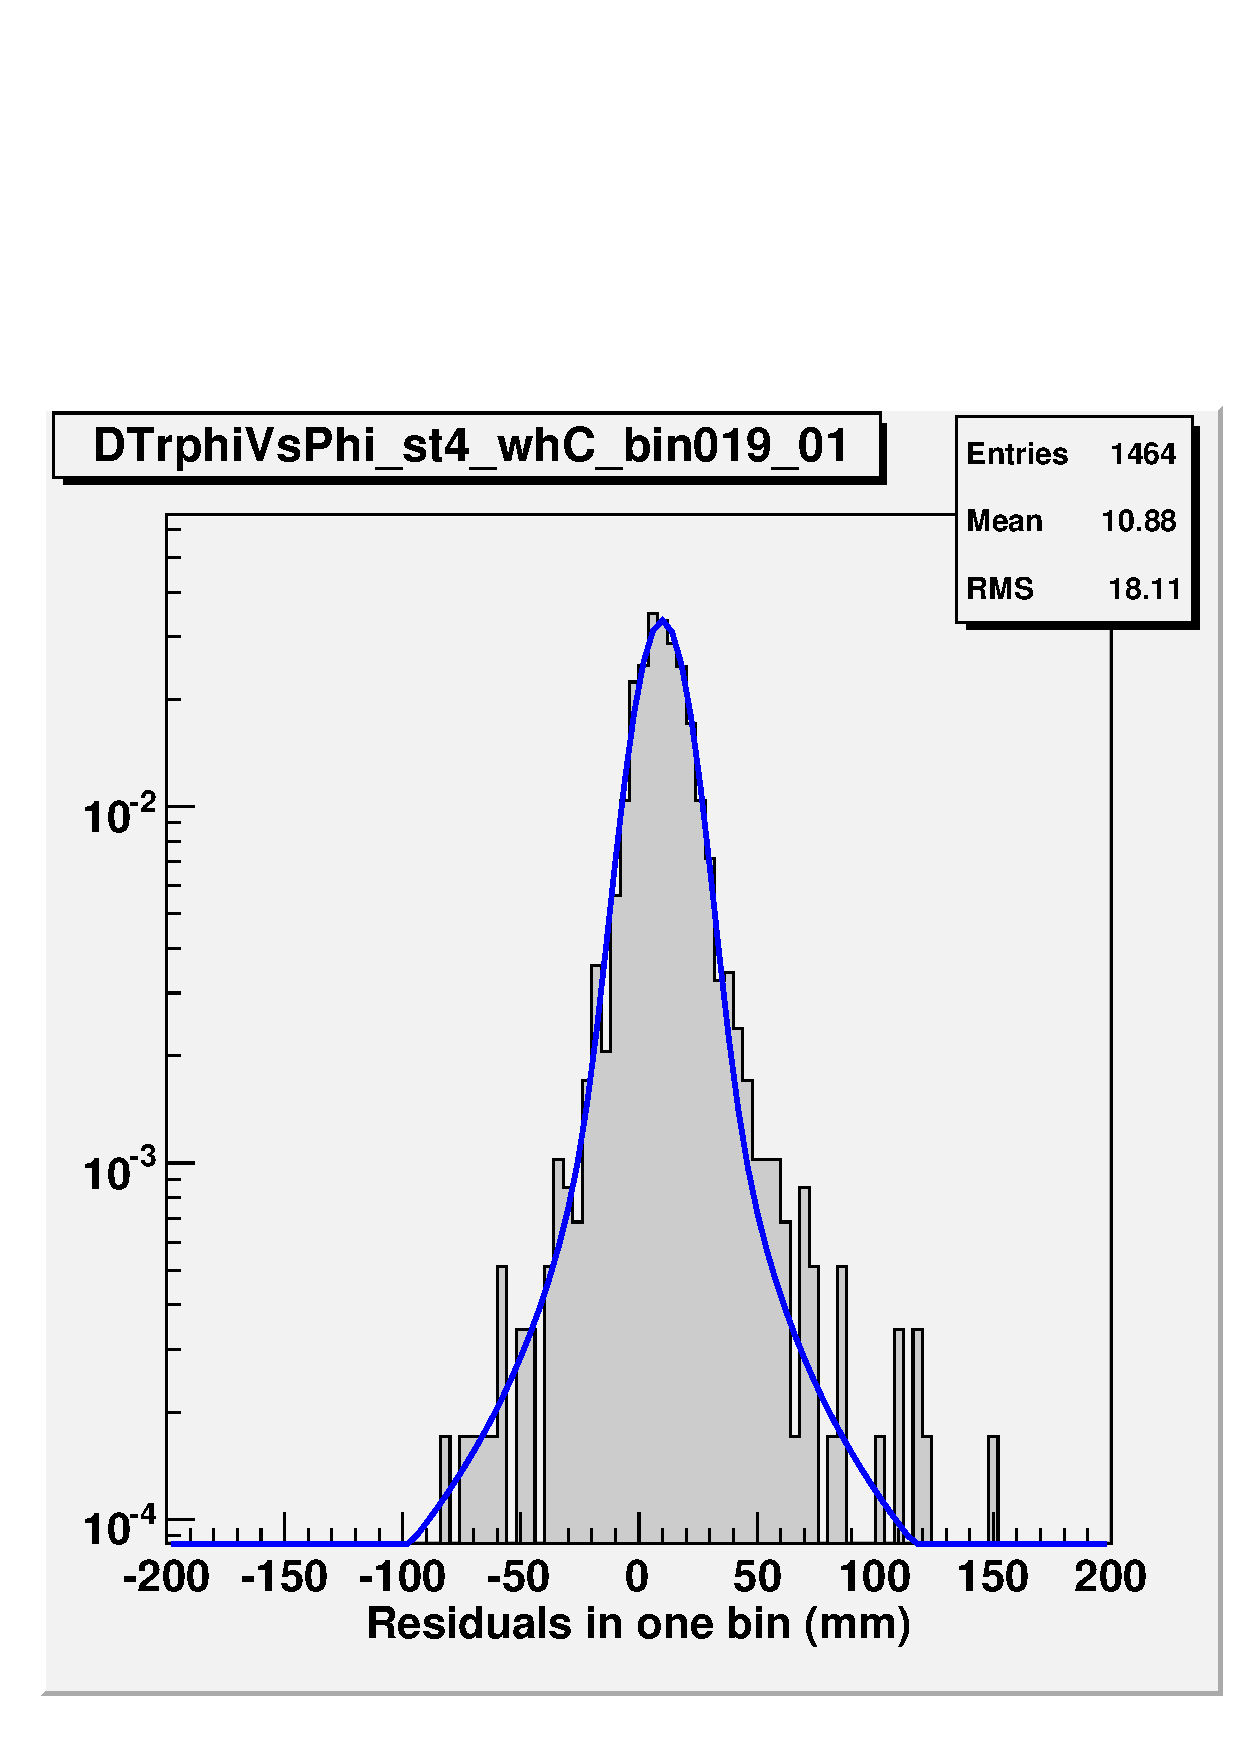
\includegraphics[width=\linewidth]{fitfunction.pdf}
\end{columns}

\begin{itemize}
\item regular mean ($\sum x_i/N$) is mathematically \\ equal to the center of an unbinned Gaussian fit
\item this is a small generalization: only added tails
\item tails de-emphasize outliers because power-law contributes far less to log likelihood than exponential
\end{itemize}
\end{frame}

\begin{frame}
\frametitle{Effect of biases in track source}

\begin{itemize}
\item Track source is treated as an absolute reference; any biases would be communicated to the muon geometry
\item Virtue of cosmic rays: wide distribution of entrance angles effectively averages over tracking volume
\begin{itemize}
\item distribution of biases must be ``low multipoles'' \\ e.g.\ $\sin\phi$, $\sin 2\phi$, $z$, $z^2$, $z^3$ etc.
\end{itemize}
\item Extenal biases cannot know anything about the chamber boundaries
\item Opportunity to X-ray tracker and identify sources:
\end{itemize}

\mbox{\hspace{-0.5 cm}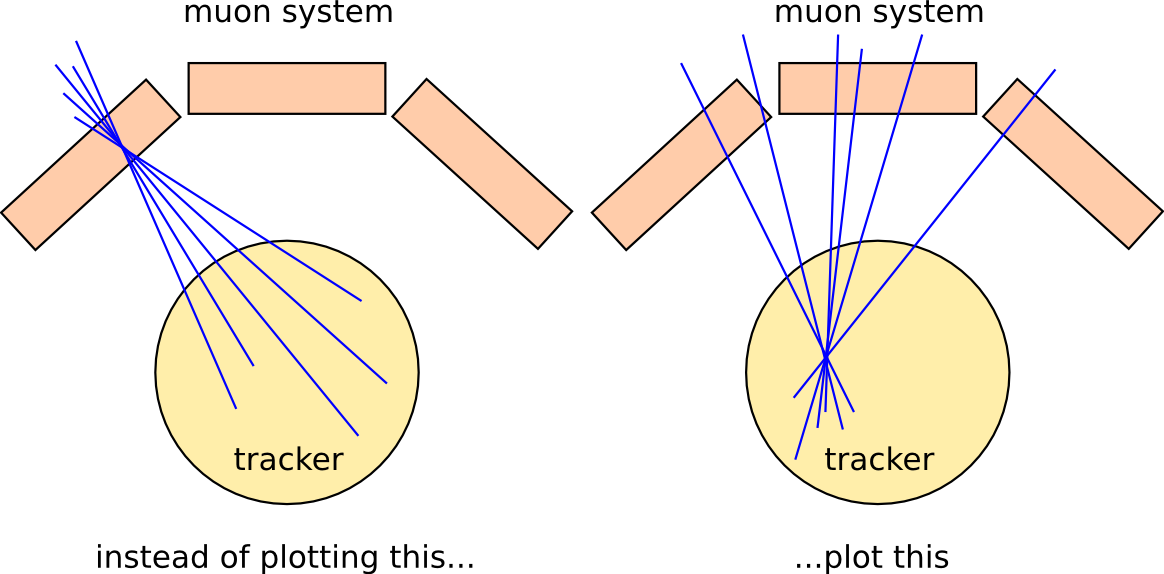
\includegraphics[height=3.8 cm]{tracker_xray.png} \hspace{0.3 cm} 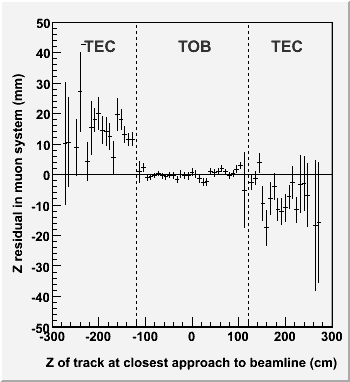
\includegraphics[height=4.2 cm]{zresid_from_tracker_outerbottom.png}}
\end{frame}

\begin{frame}
\frametitle{Effect of biases in track source}
\begin{itemize}
\item Dropping all tracks with TID and TEC hits reduces a

\vspace{0.1 cm}
$z_{\mbox{\scriptsize residuals}} \propto \big(\sin 2\phi\big) \big(z\big)$ trend in track source

\vspace{0.1 cm}
\item Wheels $\pm$2 most affected by TEC; excluding these tracks limits our alignment to inner wheels
\begin{itemize}
\item follow-up with standAloneMuon alignment of wheels $\pm$2 using inner wheels as a reference (part of plan on page~2)
\end{itemize}
\end{itemize}
\begin{center}
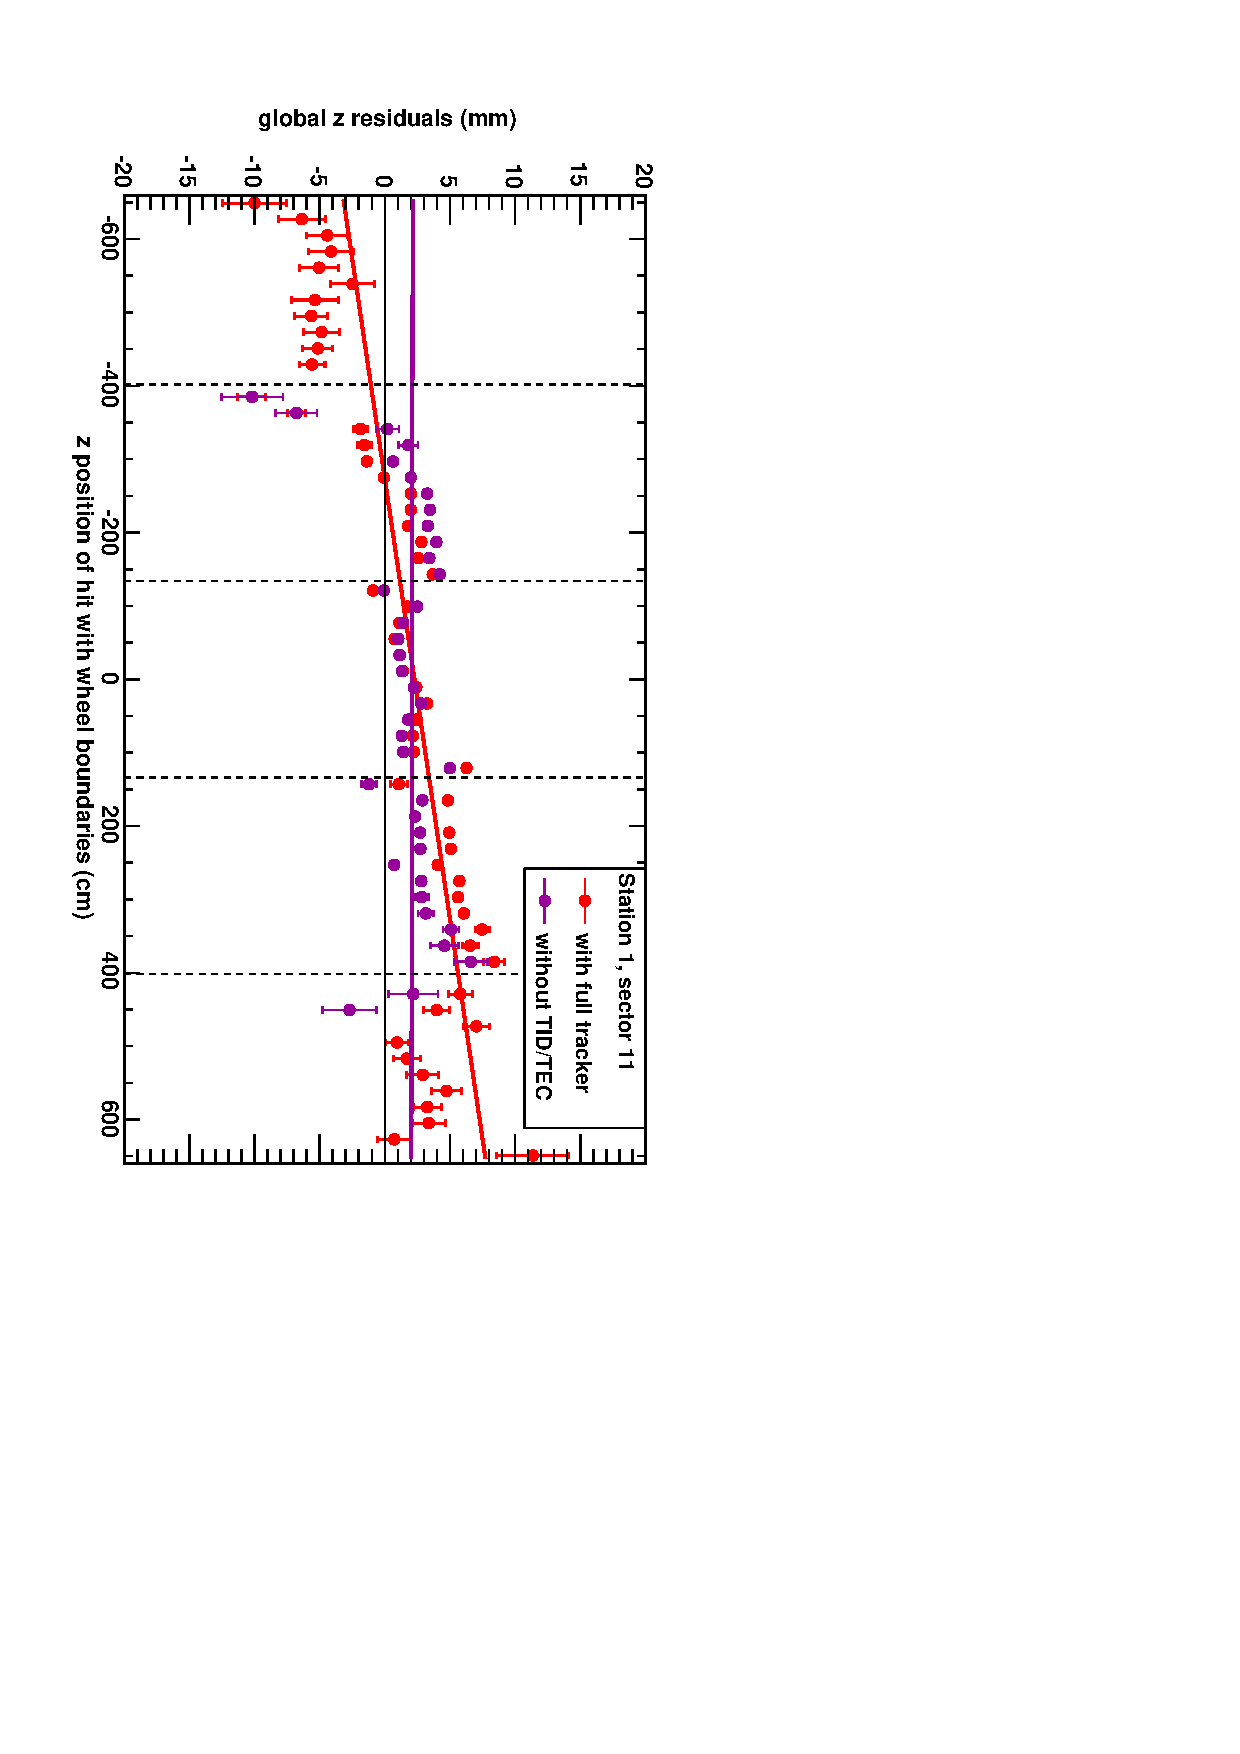
\includegraphics[height=0.9\linewidth, angle=90]{trackbias_demo.pdf}
\end{center}
\end{frame}

\begin{frame}
\frametitle{Effect of non-uniform distribution}

\vspace{-0.7 cm}
\mbox{\hspace{0.5 cm}\begin{columns}
\column{\linewidth}

\vspace{0.6 cm}
\begin{itemize}\setlength{\itemsep}{0.35 cm}
\item Muon chambers are large and cosmic ray distribution is not uniform
\item Chambers with angular \\ misalignments can \\ legitimately have linear \\ trends in the residuals
\item Chamber offset should be calculated by the intersection of \mbox{this trend at\hspace{-0.5 cm}} the center of the chamber, not the center of mass of the \mbox{source of tracks\hspace{-1 cm}}
\item Divide each chamber into four bins, perform simple average
\end{itemize}

\column{0.5\linewidth}
\hspace{-\linewidth}
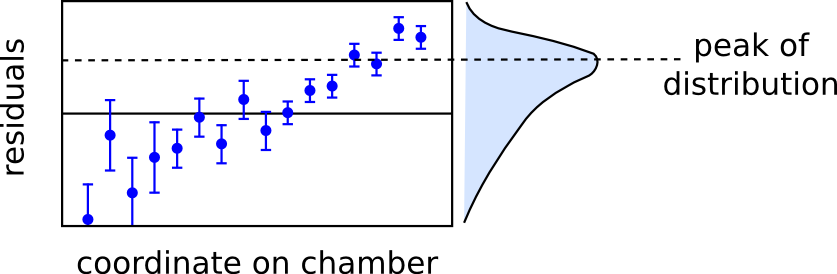
\includegraphics[width=\linewidth]{nonuniform_explanation.png}
\end{columns}}

\vspace{0.3 cm}
\begin{columns}
\column{0.4\linewidth}
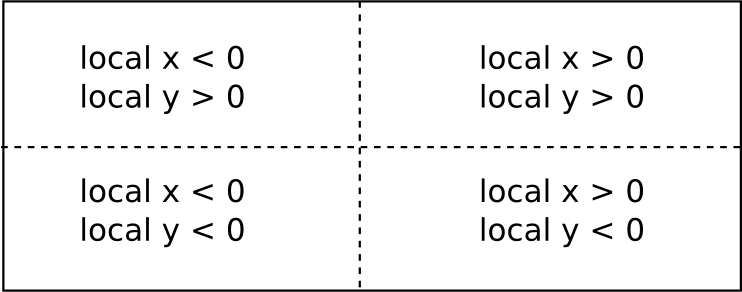
\includegraphics[width=\linewidth]{four_regions.png}

\column{0.6\linewidth}
\begin{itemize}
\item Similar to charge-binning for $\vec{B}$-field control (total of 8 bins)
\item However, this relies on approximation that distribution of tracks is linear
\end{itemize}
\end{columns}
\end{frame}

\begin{frame}
\frametitle{Alignment presented here}

\begin{itemize}
\item Align individual chambers, rather than wheels

\item Three degrees of freedom: local $x$, $y$, $\phi_z$

\begin{itemize}\setlength{\itemsep}{0.1 cm}
\item<1-| alert@1> \textcolor{red}{local $x$:} \textcolor{black}{offset in global $r\phi$ residuals}
\item<1-| alert@1> \textcolor{red}{local $y$:} \textcolor{black}{offset in global $z$ residuals (first test)}
\item local $z$: linear trend in $R_{r\phi}$ vs.\ $\phi$ and $R_{z}$
  vs.\ $z$

(because globalMuons are constrained to originate in tracker)
\item $\phi_x$: trend in $R_{z}$ vs.\ $z$ only, but second-order
\item $\phi_y$: trend in $R_{r\phi}$ vs.\ $\phi$ only, but second-order
\item<1-| alert@1> \textcolor{red}{$\phi_z$:} \textcolor{black}{linear trend in $R_{r\phi}$ vs.\ $z$ and $R_{z}$ vs.\ $\phi$}
\end{itemize}

\item Only accept chambers in which all 8 bins were successfully fitted with at least 30 ``hits'' each (averages of 1-D residuals in a chamber on a track)

\item Input muon alignment/calibration: from CRAFT\_ALL\_V4 \\ (first re-processing, includes layer and superlayer corrections)

\item Input tracker alignment/calibration: new version for second re-processing, including layer-by-layer Lorentz angle corrections
\end{itemize}
\end{frame}

\begin{frame}
\frametitle{Track-based validation}

\begin{itemize}
\item See ``more information'' for 152 pages of plots like this one
\begin{itemize}
\item dataset is divided such that you're only ever looking at one chamber at a time
\item grey background is the raw 2-D residuals distribution
\item linear fits are only a guide for the eye, not used in alignment
\end{itemize}
\end{itemize}

\vspace{-0.4 cm}
\begin{center}
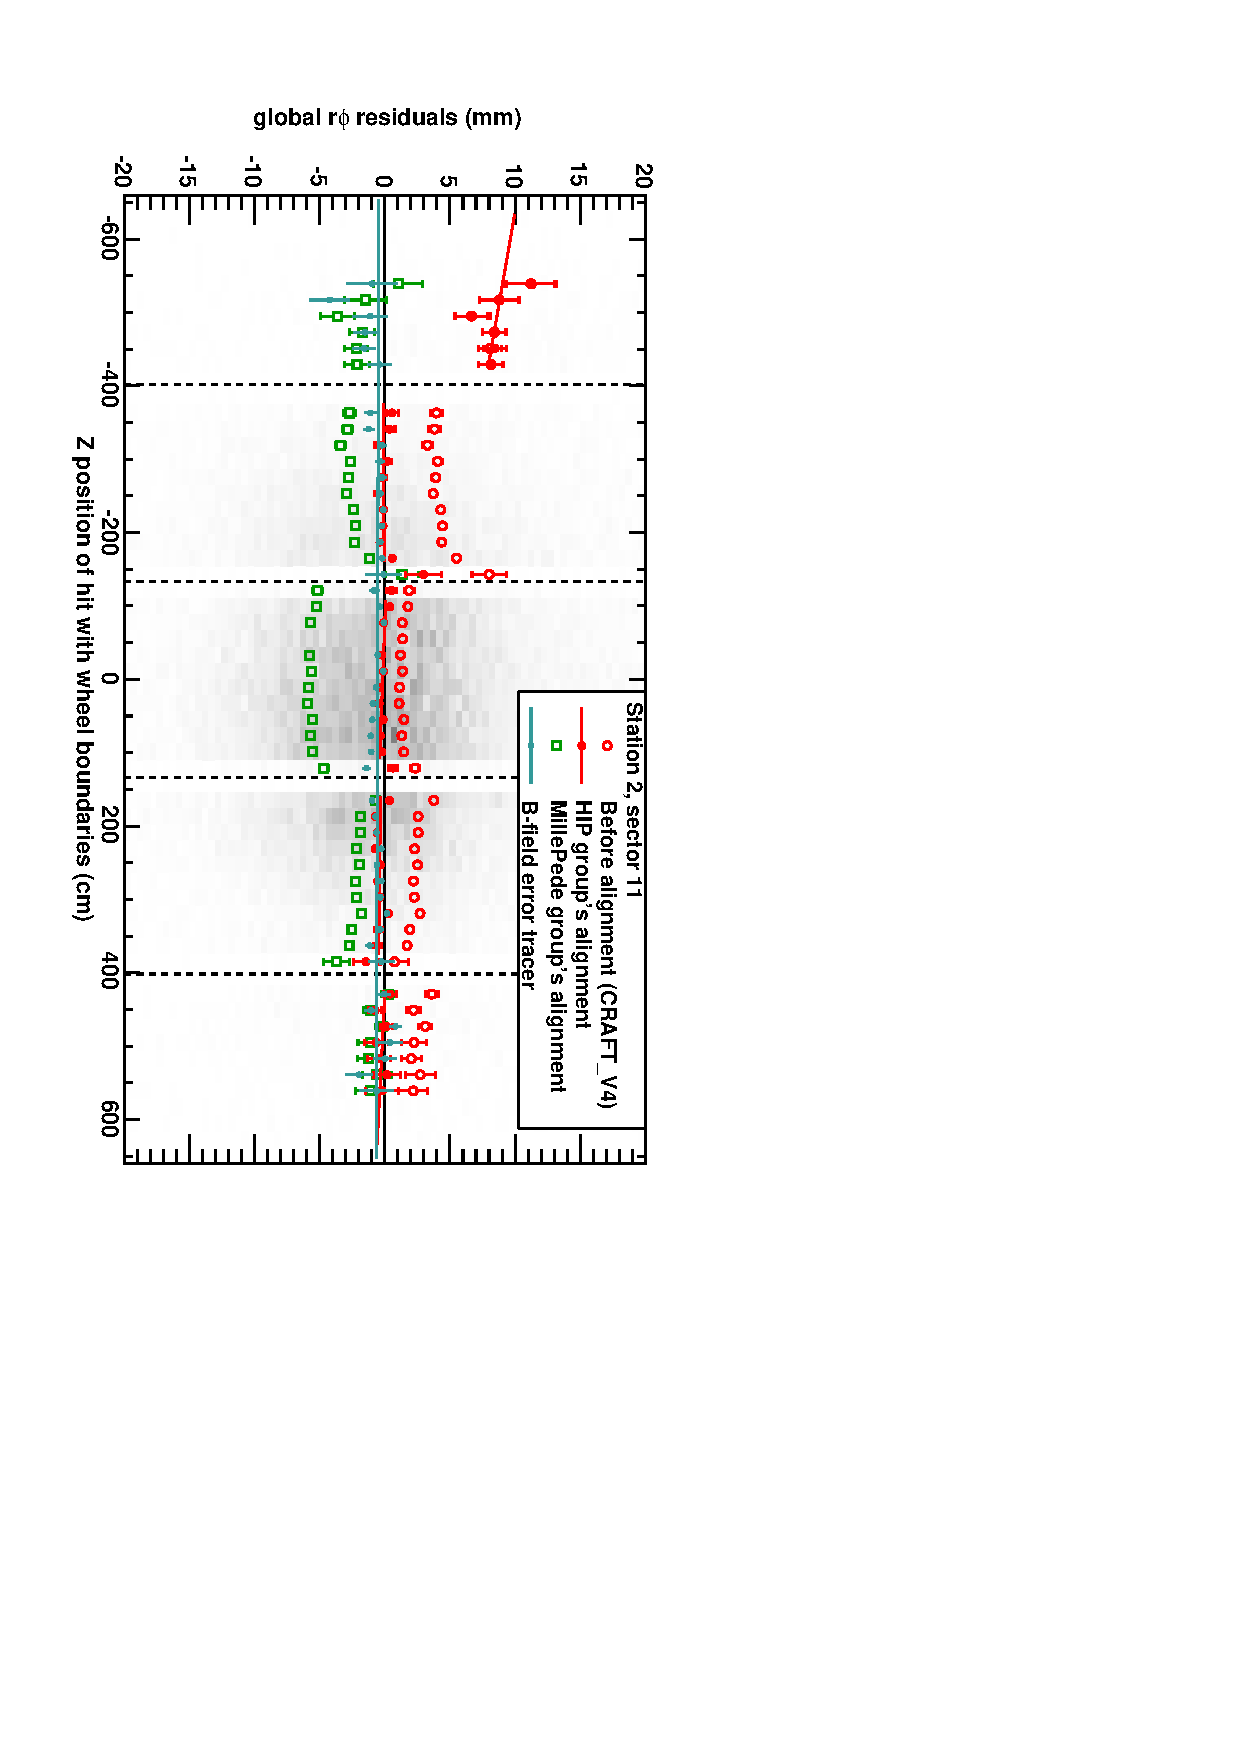
\includegraphics[height=0.95\linewidth, angle=90]{DTrphiVsZ_st2_sr11.pdf}
\end{center}

\vspace{-0.5 cm}
\begin{itemize}
\item Wheel $-$2, station~2, sector~11 didn't have enough \mbox{tracks for alignment\hspace{-1 cm}}
\end{itemize}
\end{frame}

\begin{frame}
\frametitle{Summary of residuals}

\begin{itemize}
\item To summarize, project all residuals ($p_T > 80$~GeV, all chambers)
\begin{itemize}
\item like the tracker's $\chi^2/N_{\mbox{\scriptsize dof}}$ plot, but unweighted
\item less sensitive measure of alignment, but convenient
\end{itemize}
\end{itemize}

\begin{columns}
\column{0.25\linewidth}
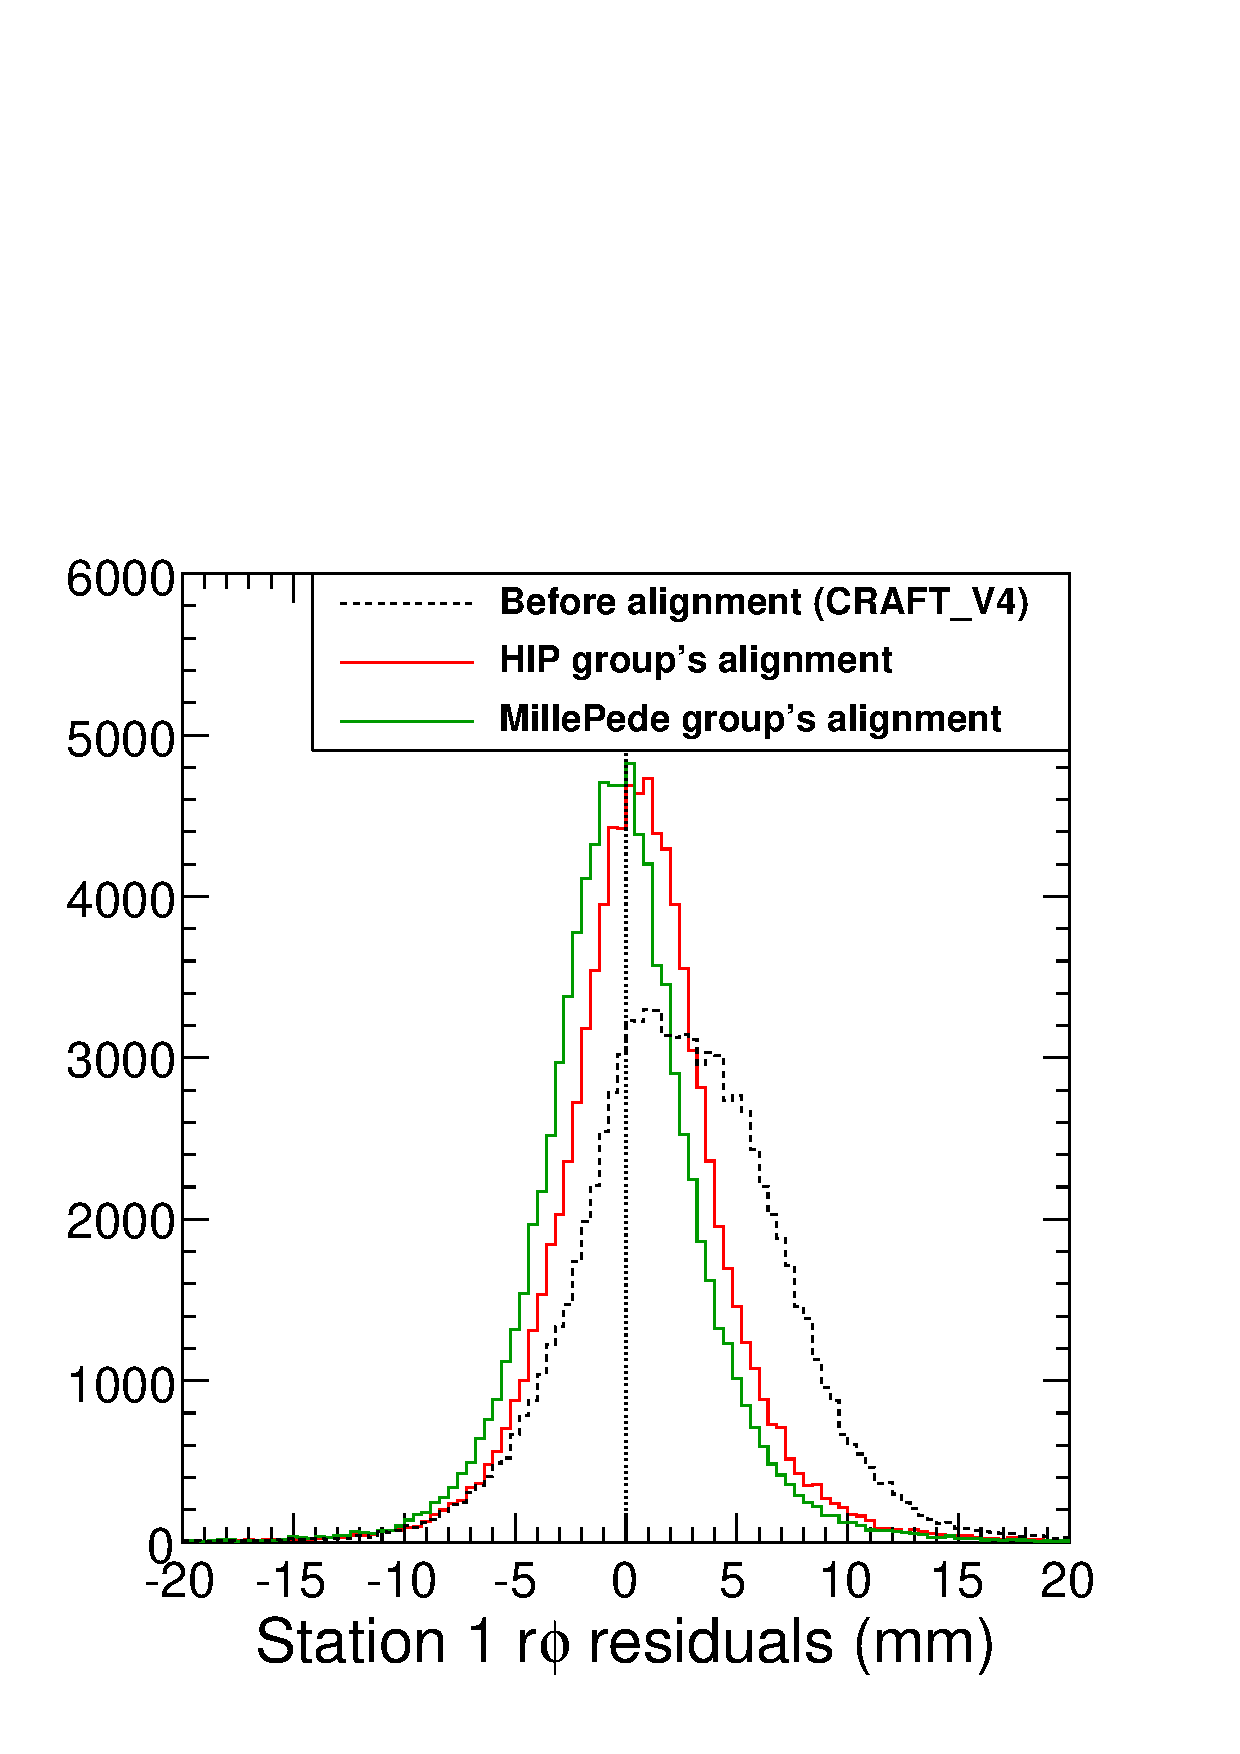
\includegraphics[width=\linewidth]{raw_station1.pdf}

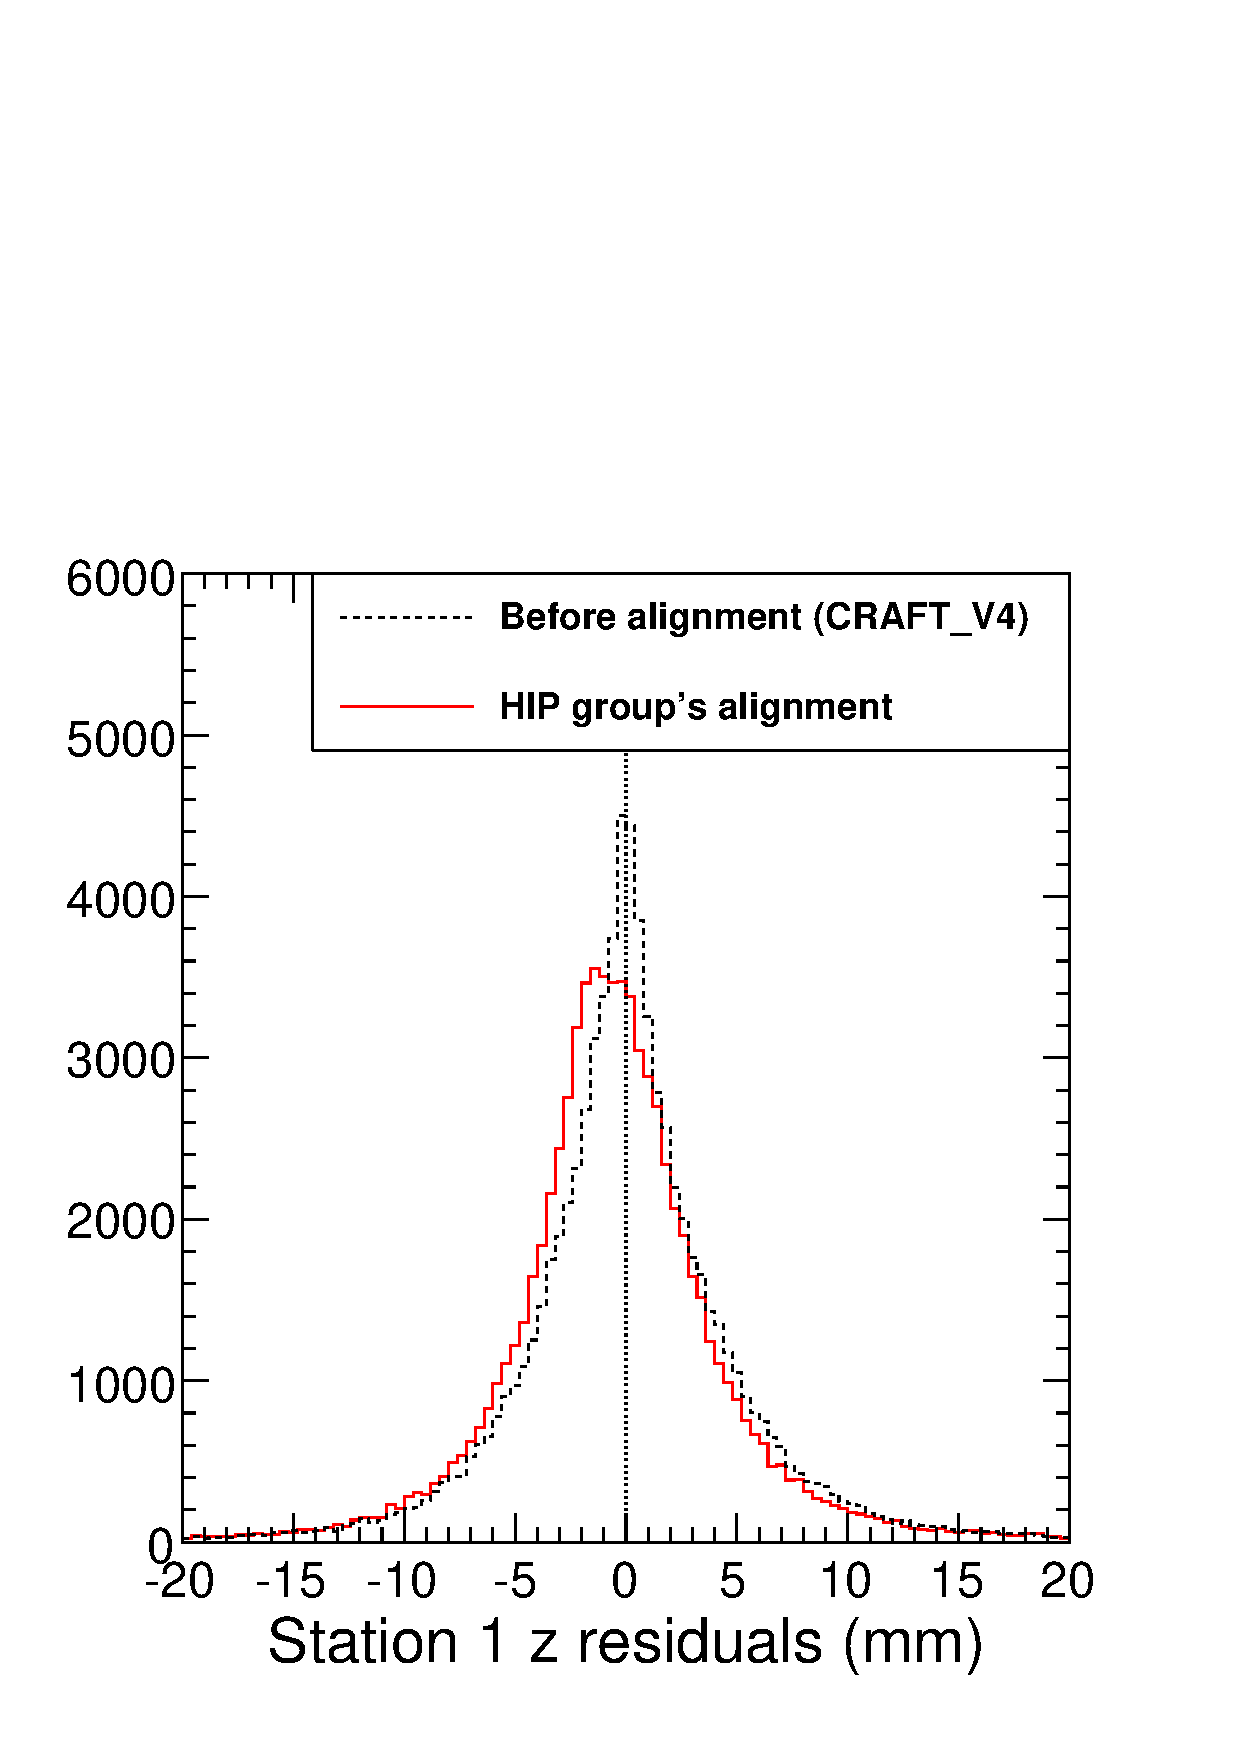
\includegraphics[width=\linewidth]{rawz_station1.pdf}

\column{0.25\linewidth}
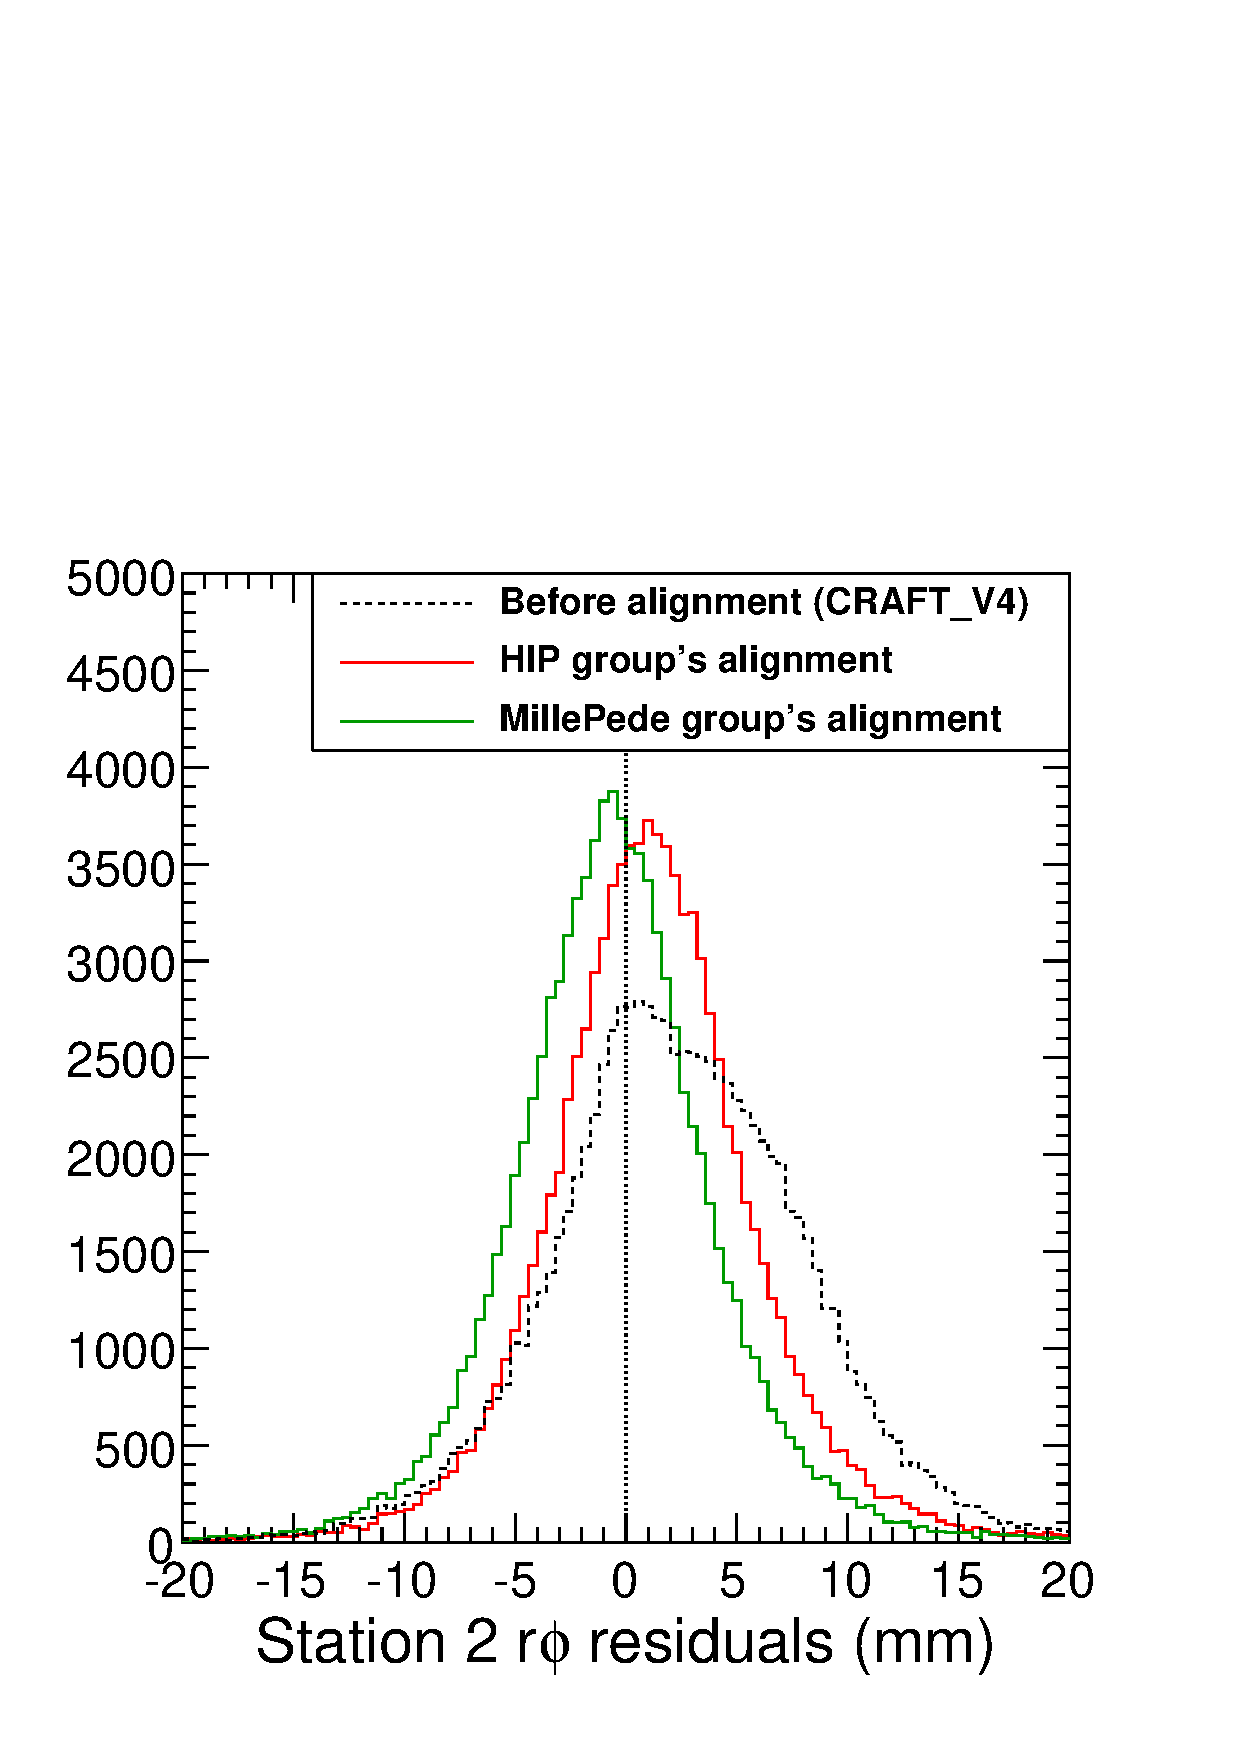
\includegraphics[width=\linewidth]{raw_station2.pdf}

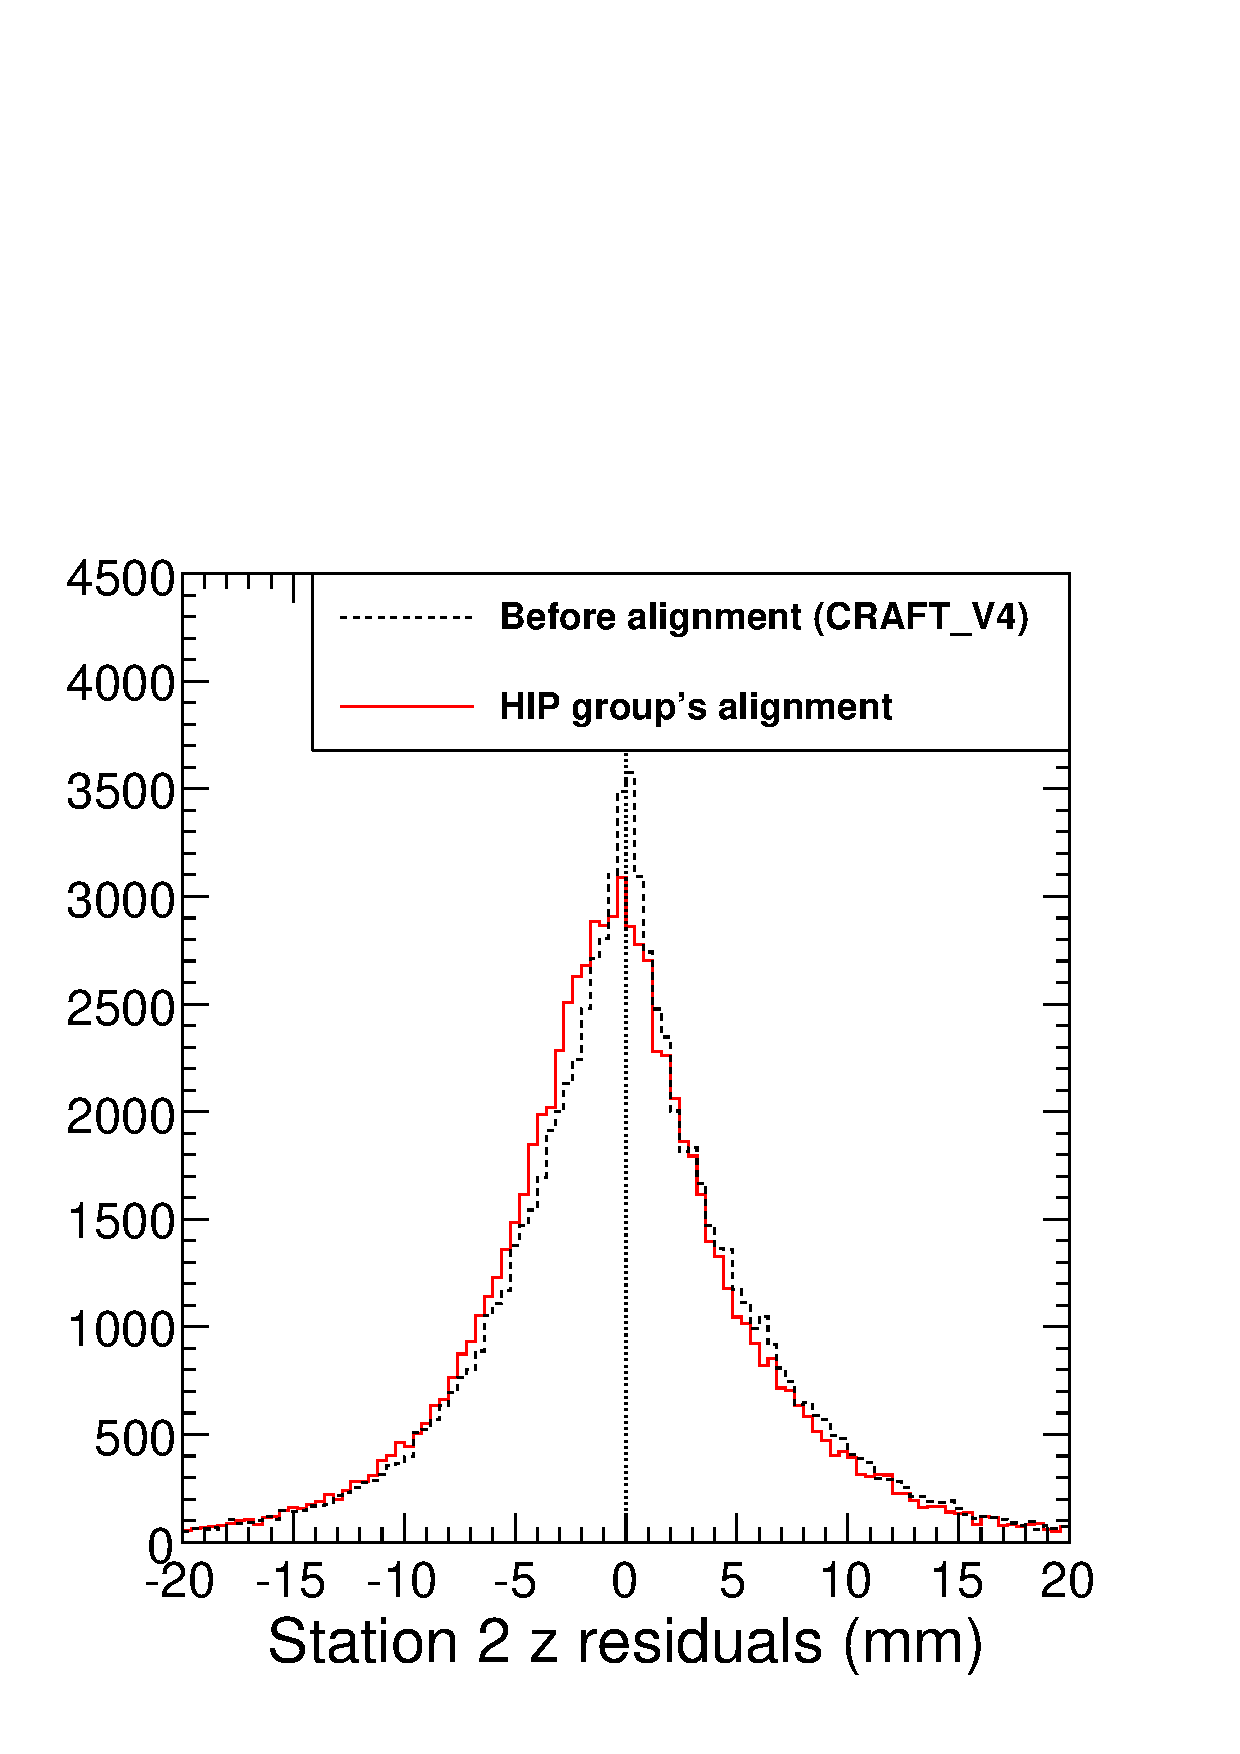
\includegraphics[width=\linewidth]{rawz_station2.pdf}

\column{0.25\linewidth}
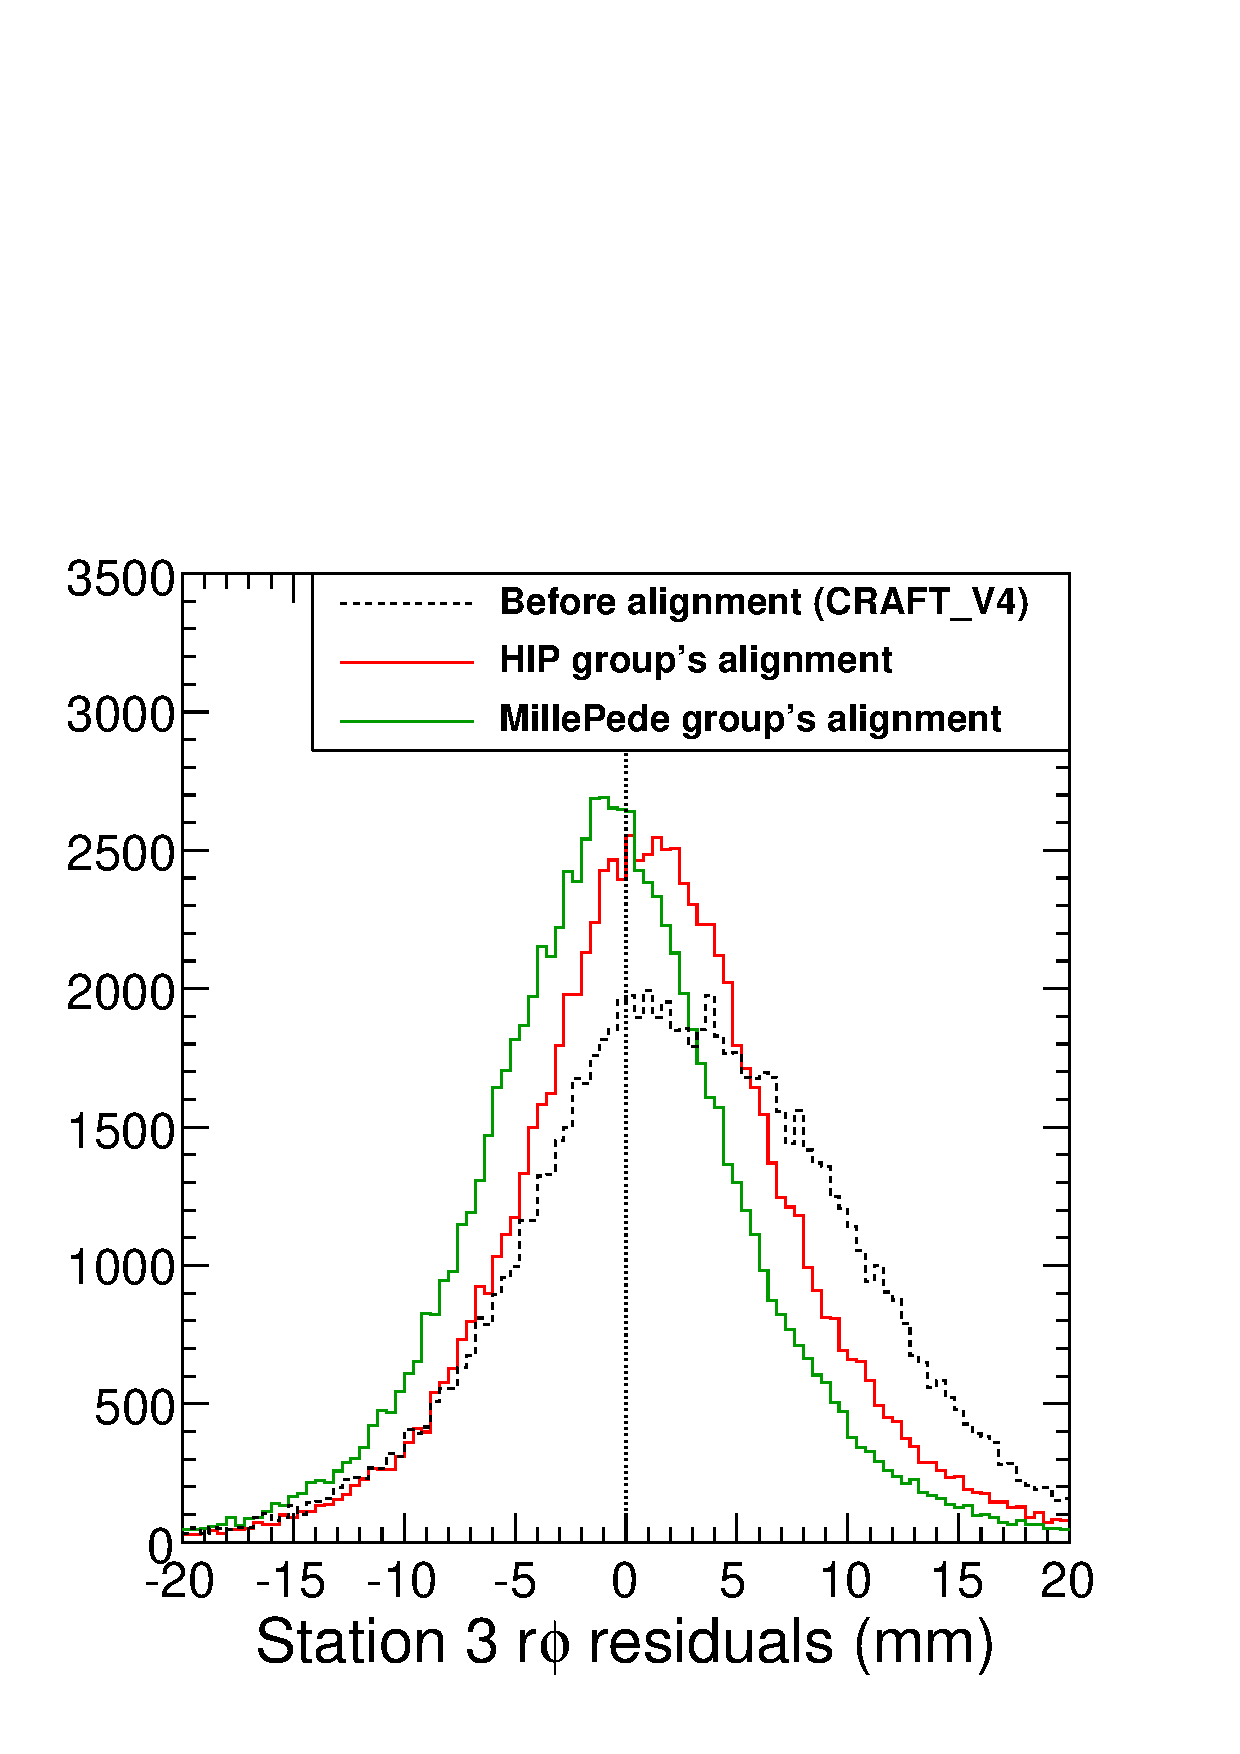
\includegraphics[width=\linewidth]{raw_station3.pdf}

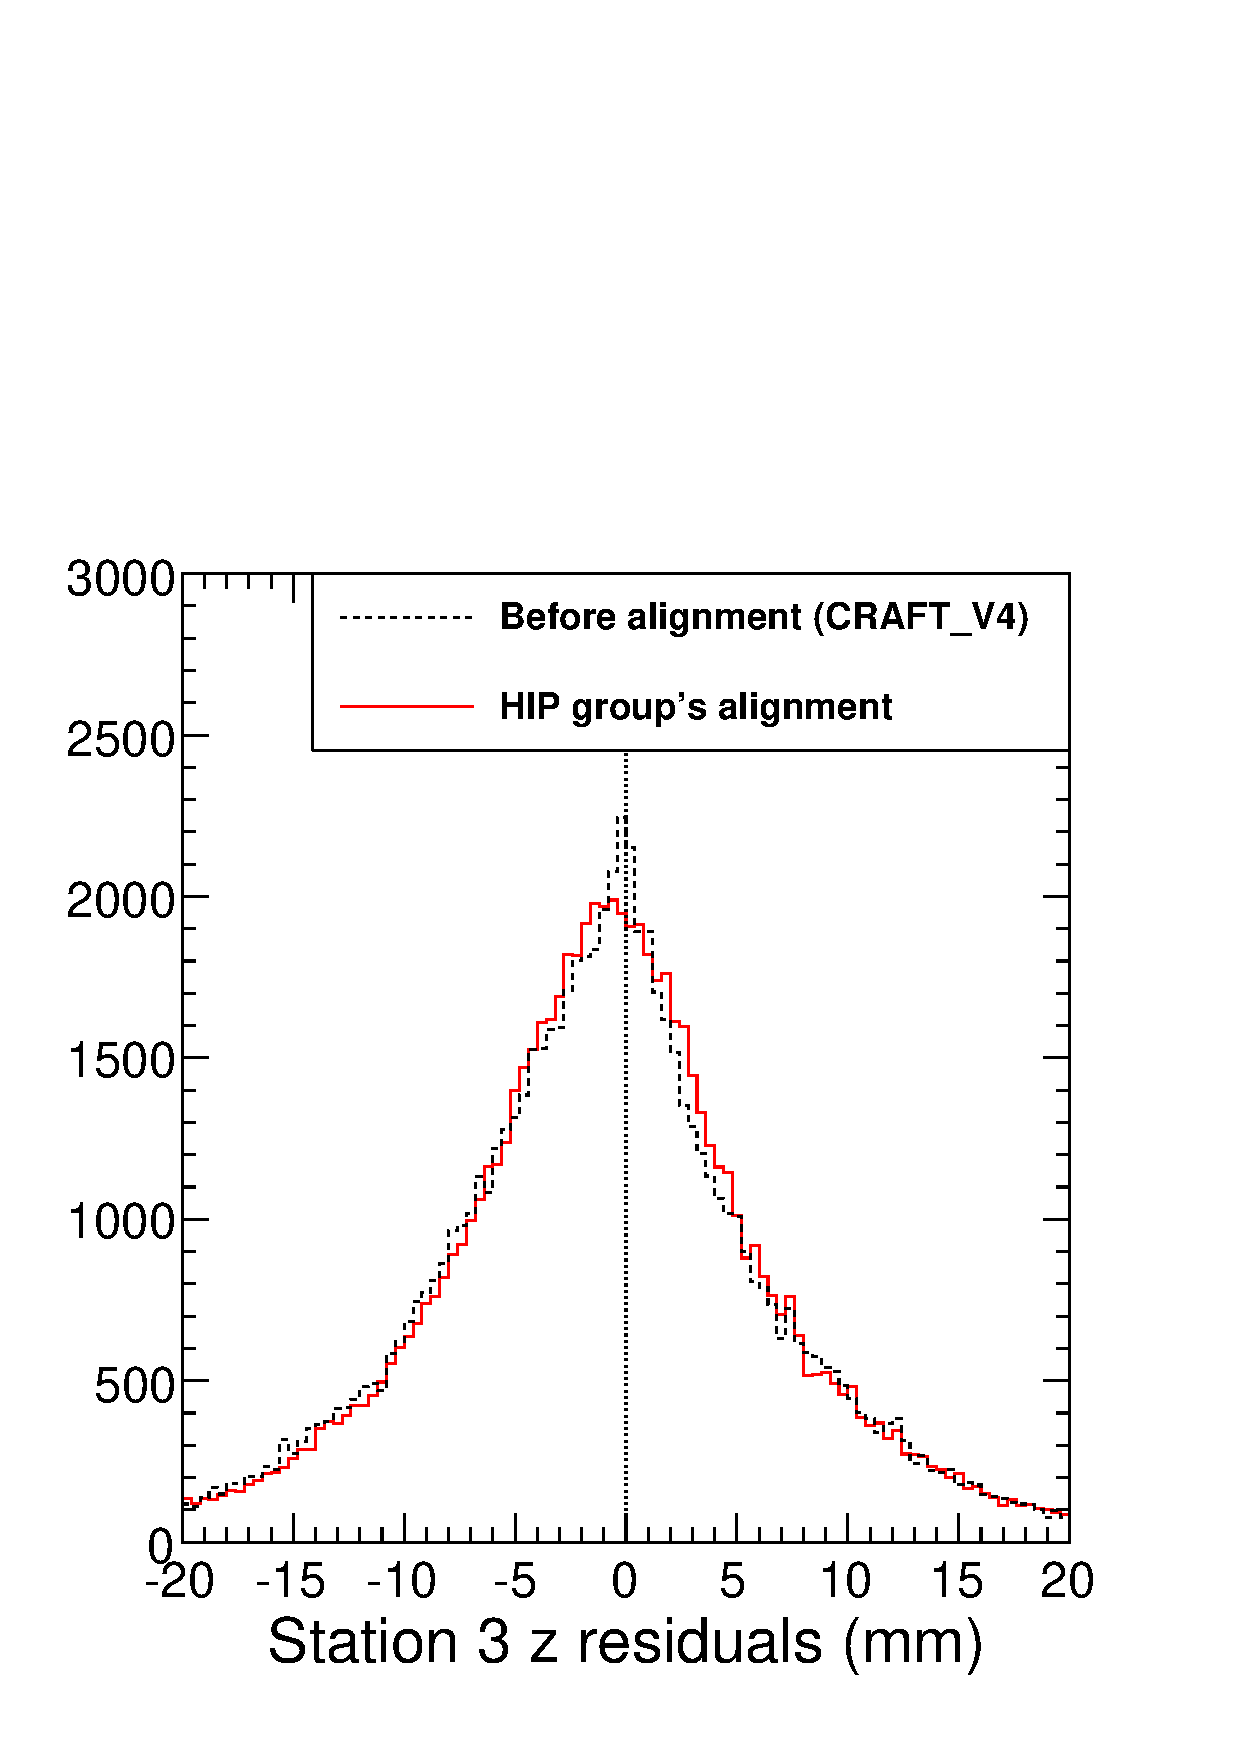
\includegraphics[width=\linewidth]{rawz_station3.pdf}

\column{0.25\linewidth}
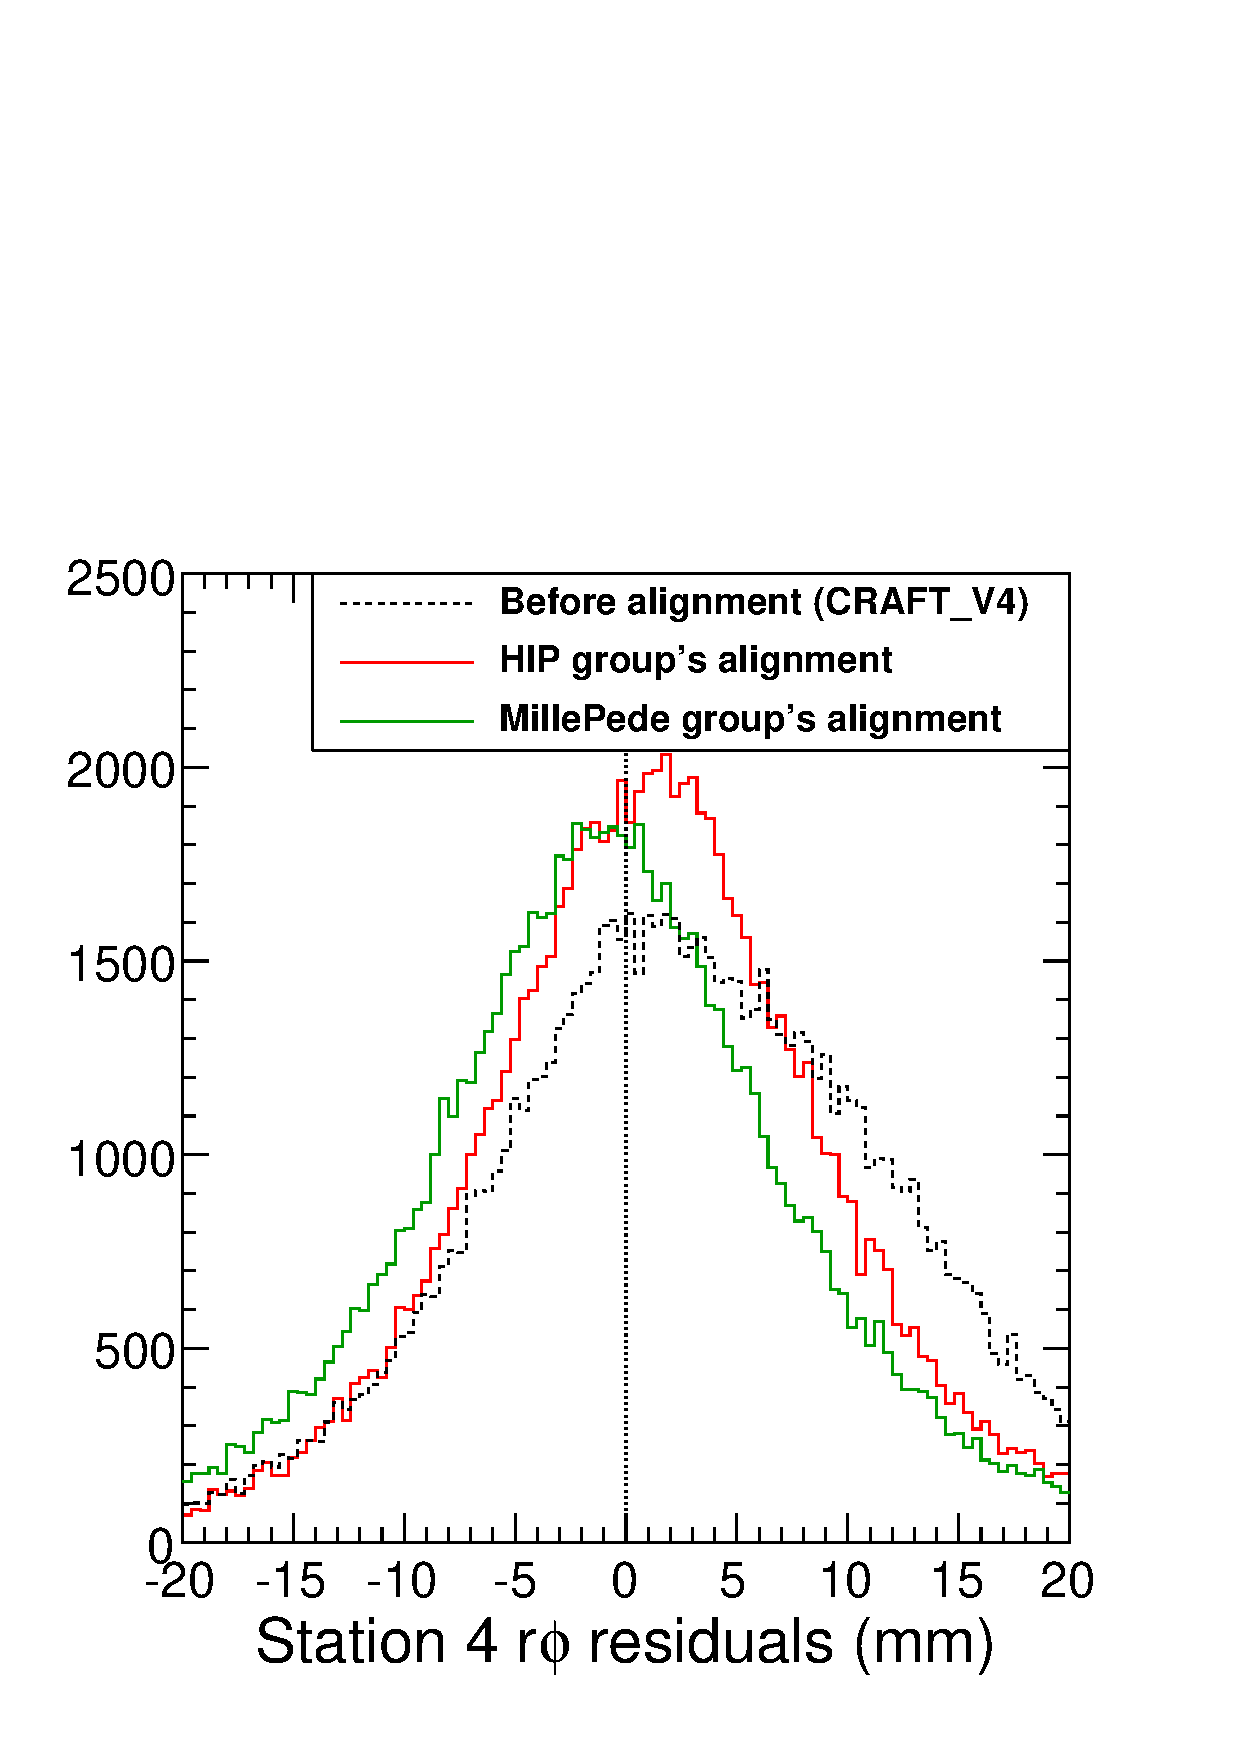
\includegraphics[width=\linewidth]{raw_station4.pdf}
\end{columns}
\end{frame}

\begin{frame}
\frametitle{Linearly-independent validation}

\begin{itemize}
\item Residuals in plots are calculated the same way as residuals \mbox{in alignment\hspace{-1 cm}}
\item Linearly-independent test: residuals differences between
  \mbox{pairs of stations\hspace{-1 cm}}

\mbox{$\mbox{difference} = \big(\mbox{st.\ 3 track} - \mbox{st.\ 3 hit}\big) - \big(\mbox{st.\ 2 track} - \mbox{st.\ 2 hit}\big)$}

\begin{itemize}\setlength{\itemsep}{0.1 cm}
\item shows {\it relative} positions of chambers; globalMuon is just a ruler
\item note zoomed vertical scale: accuracy is 1--2~mm
\item also shows $\vec{B}$-field error between the stations, not integrated
\end{itemize}
\end{itemize}

\vspace{-0.4 cm}
\begin{center}
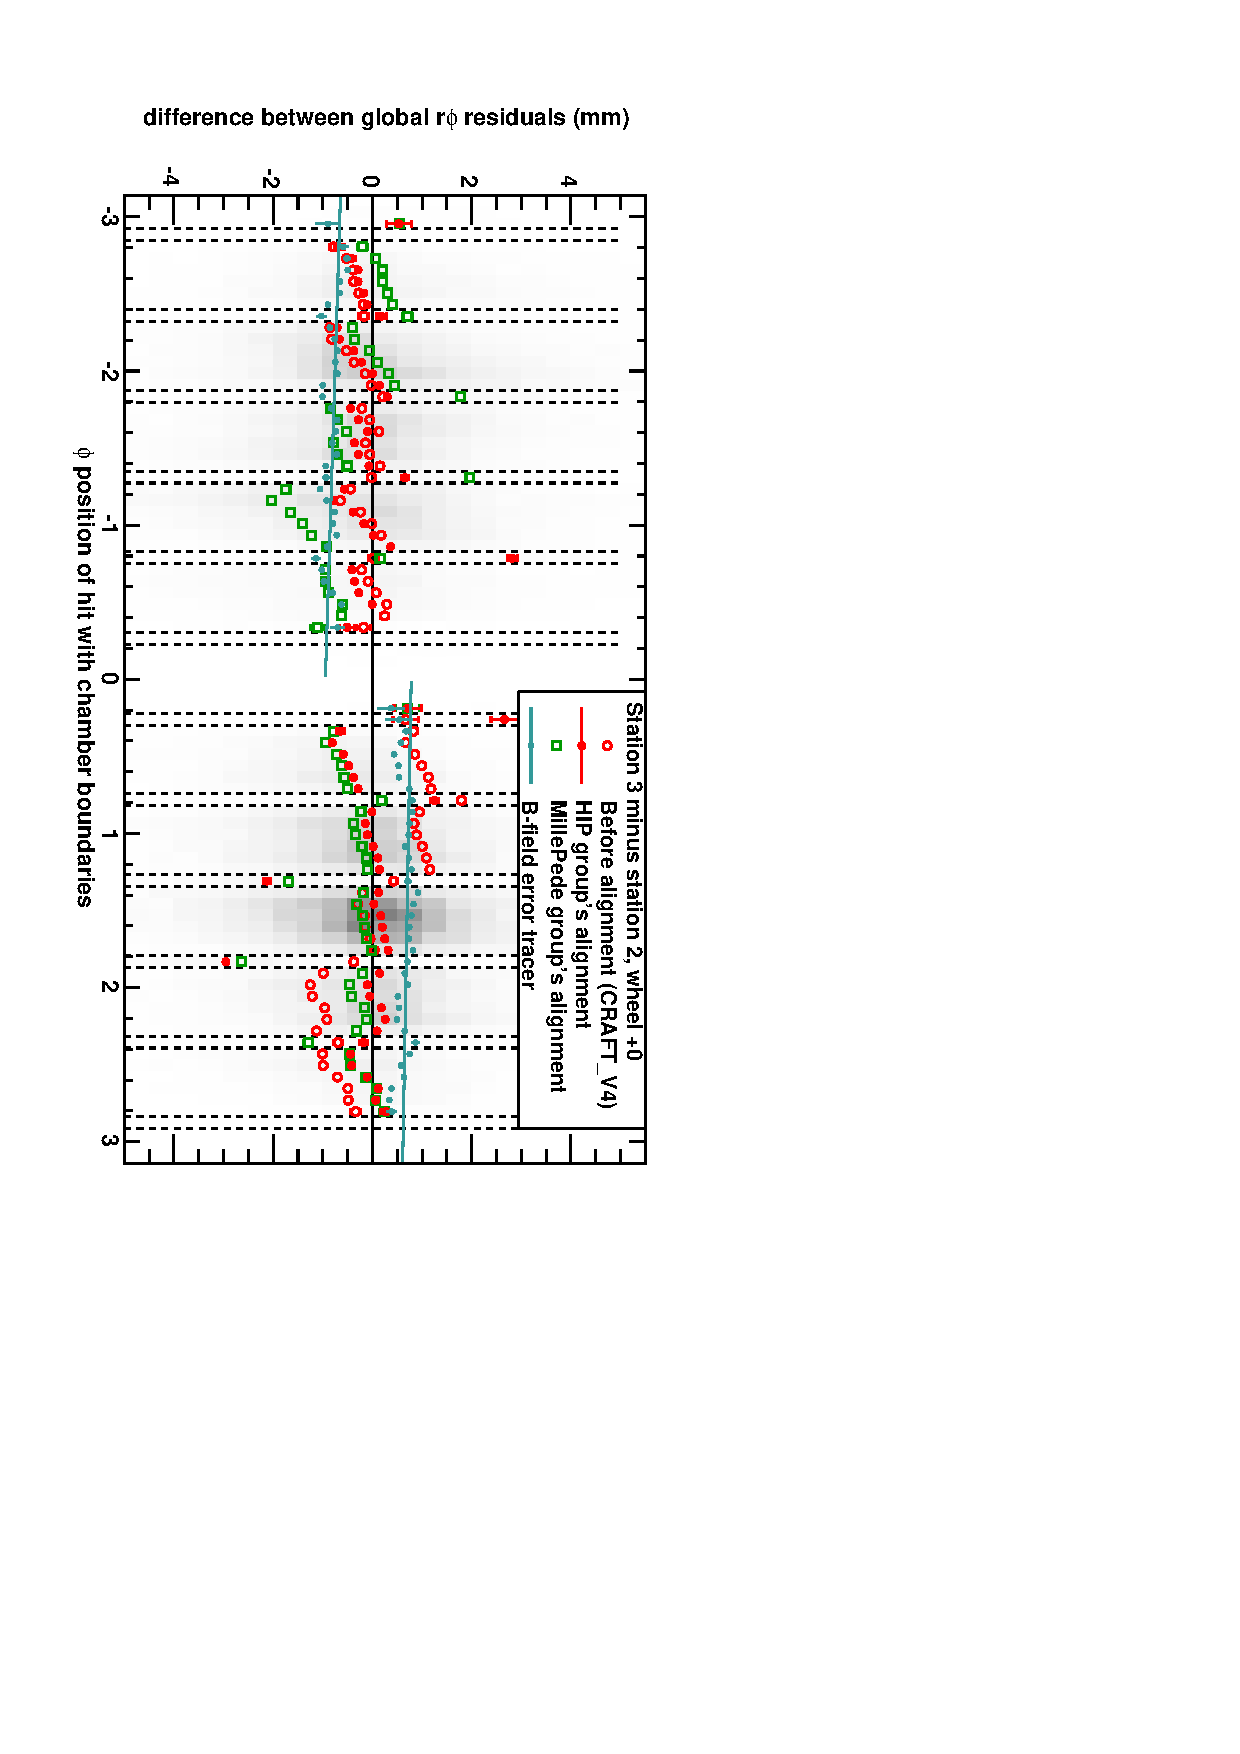
\includegraphics[height=0.95\linewidth, angle=90]{DTrphidiff23VsPhi_whC.pdf}
\end{center}
\end{frame}

\begin{frame}
\frametitle{Values of the corrections}

\begin{columns}
\column{0.35\linewidth}
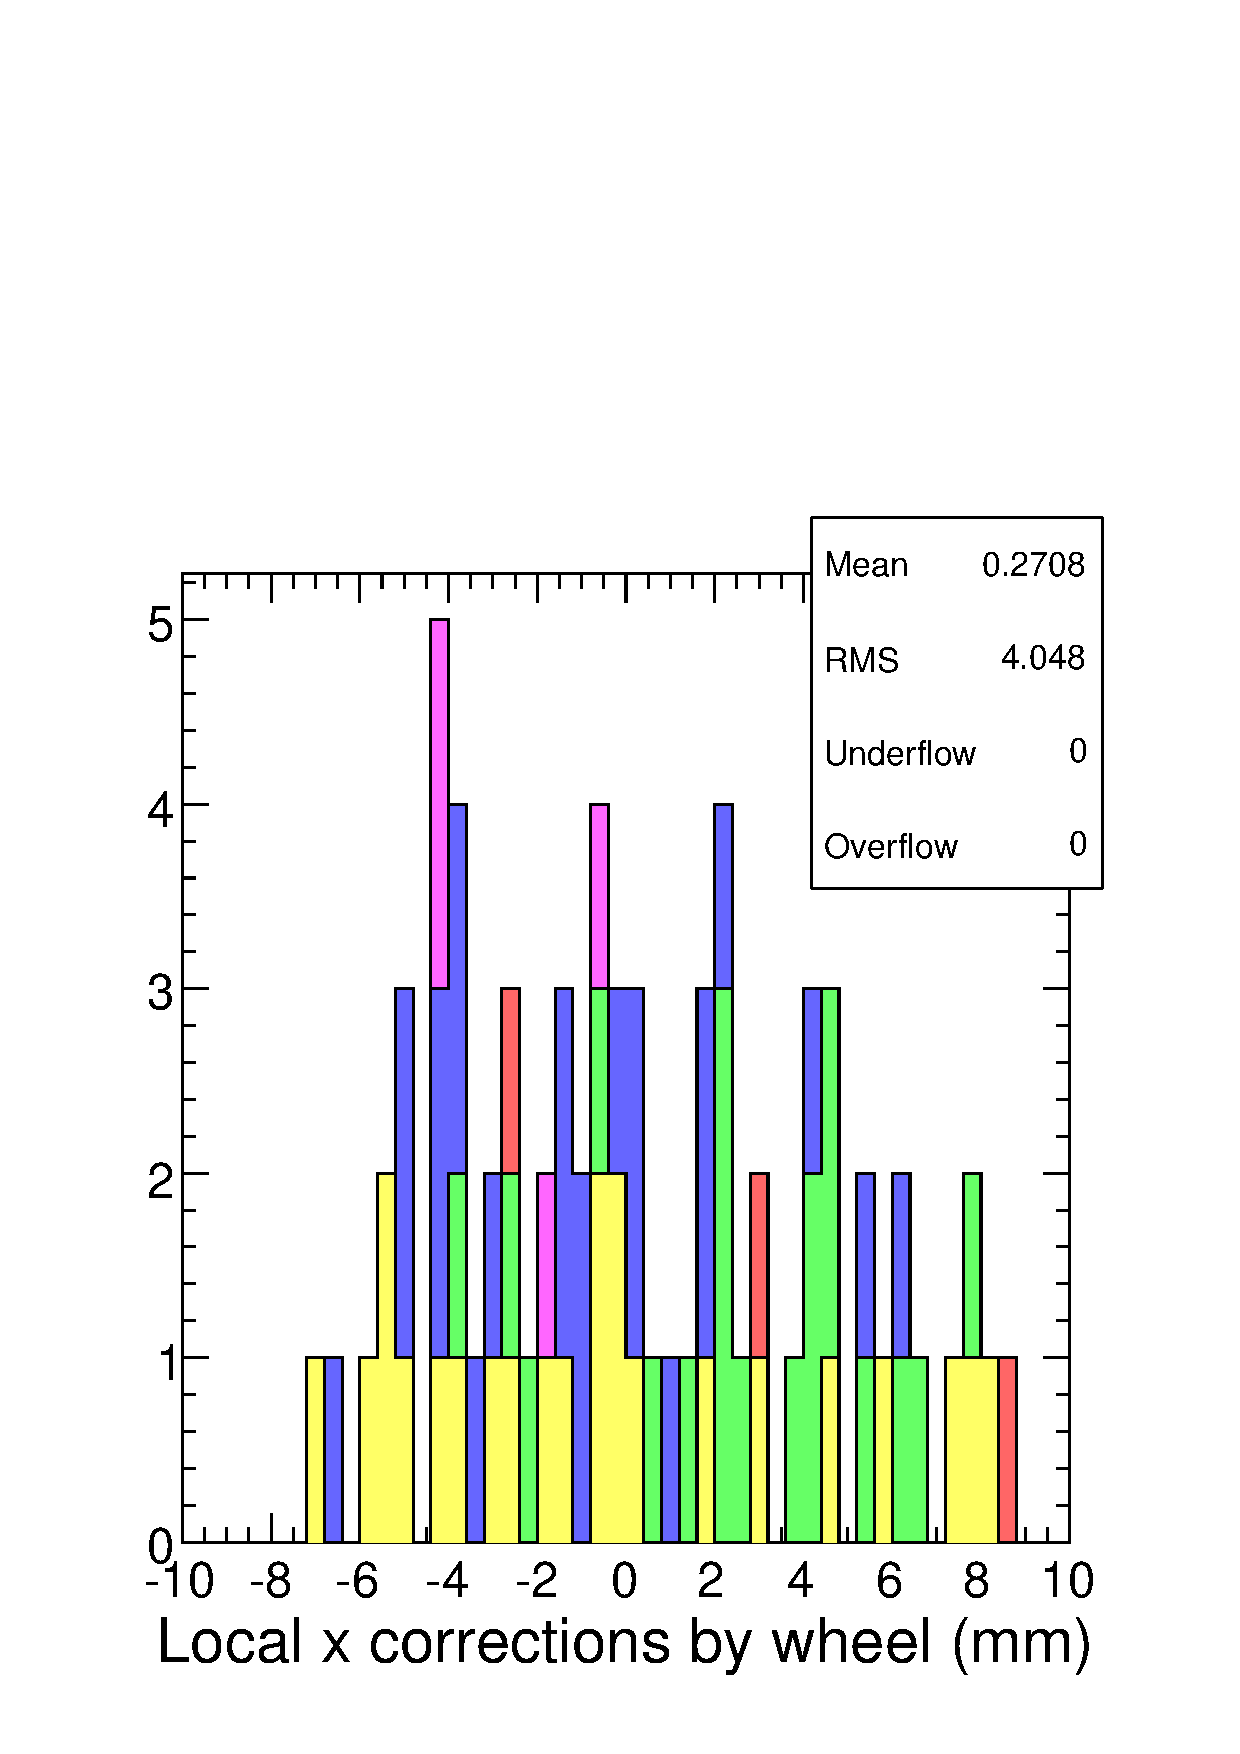
\includegraphics[width=\linewidth]{corrections_x.pdf}

\column{0.35\linewidth}
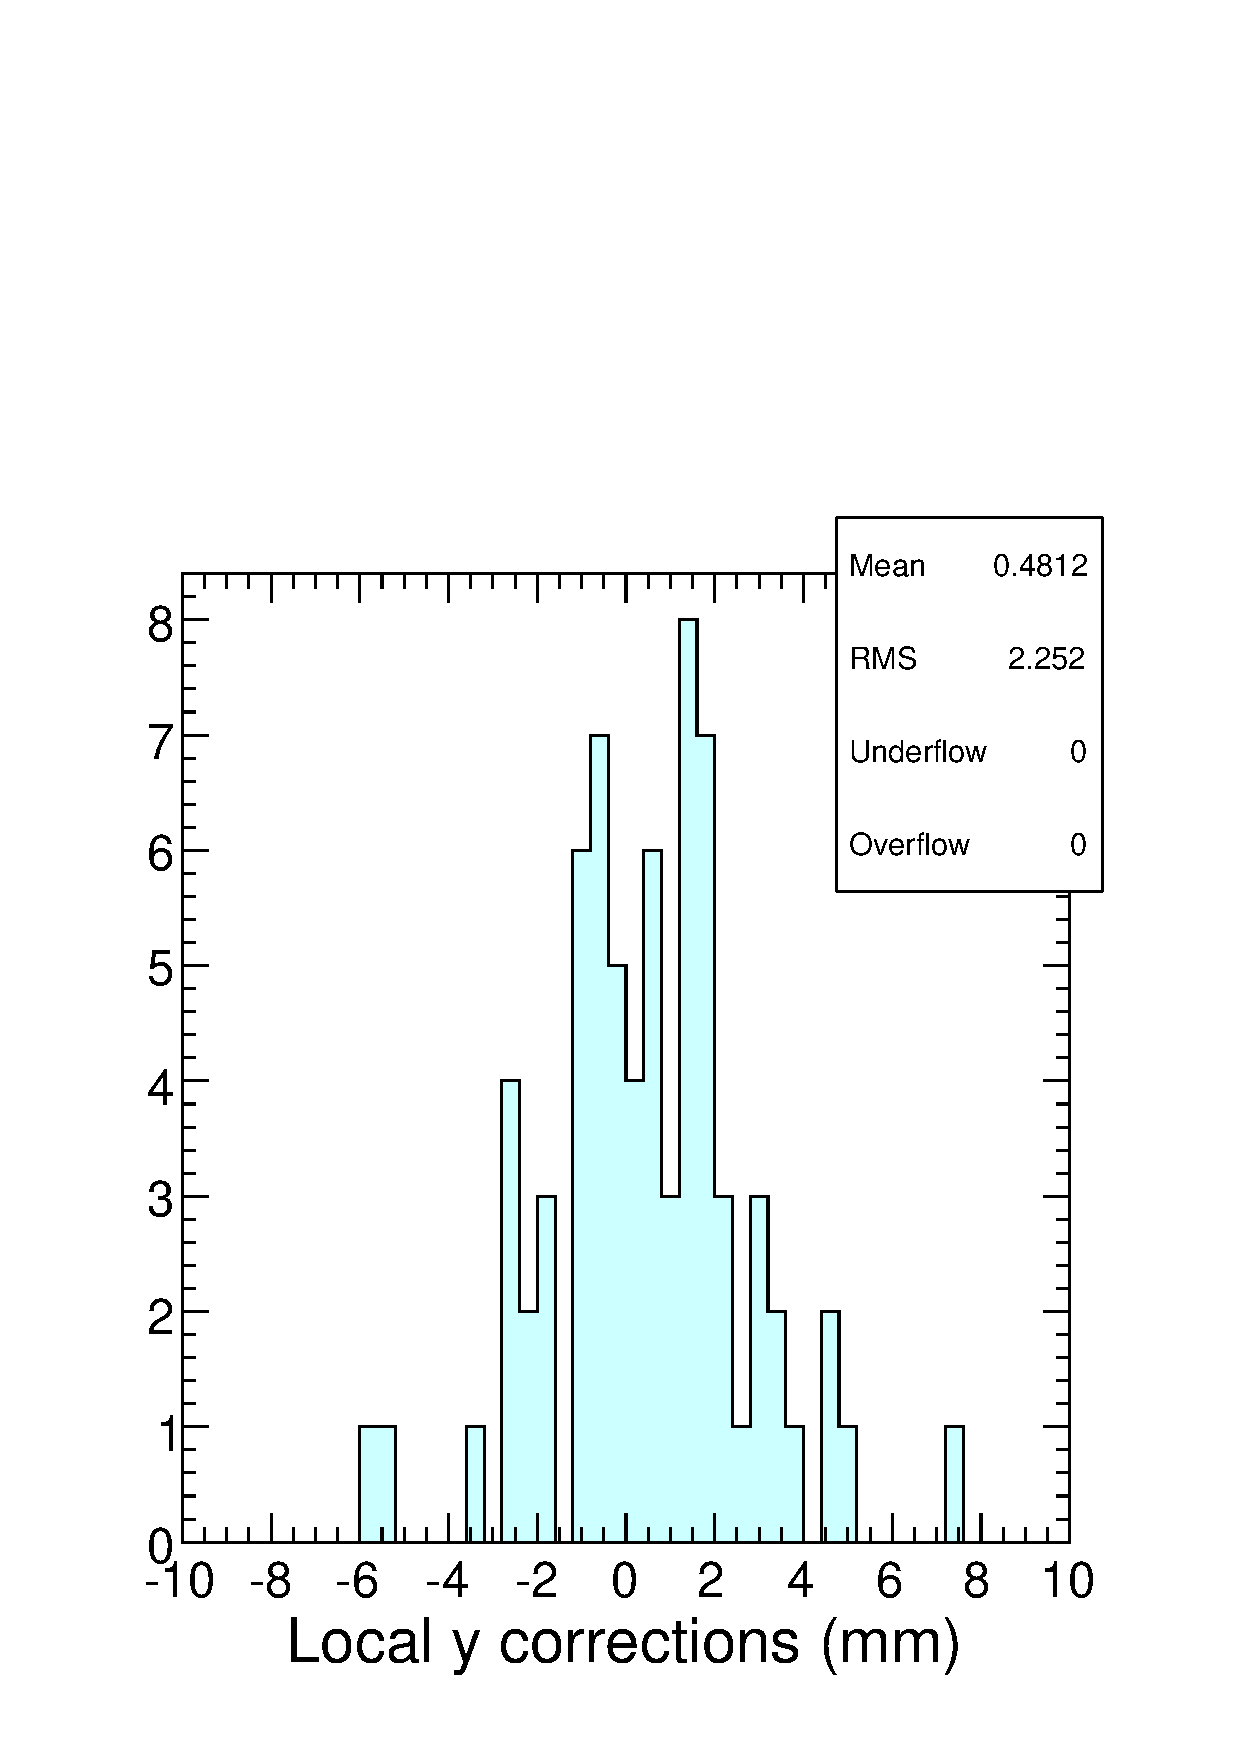
\includegraphics[width=\linewidth]{corrections_y.pdf}

\column{0.35\linewidth}
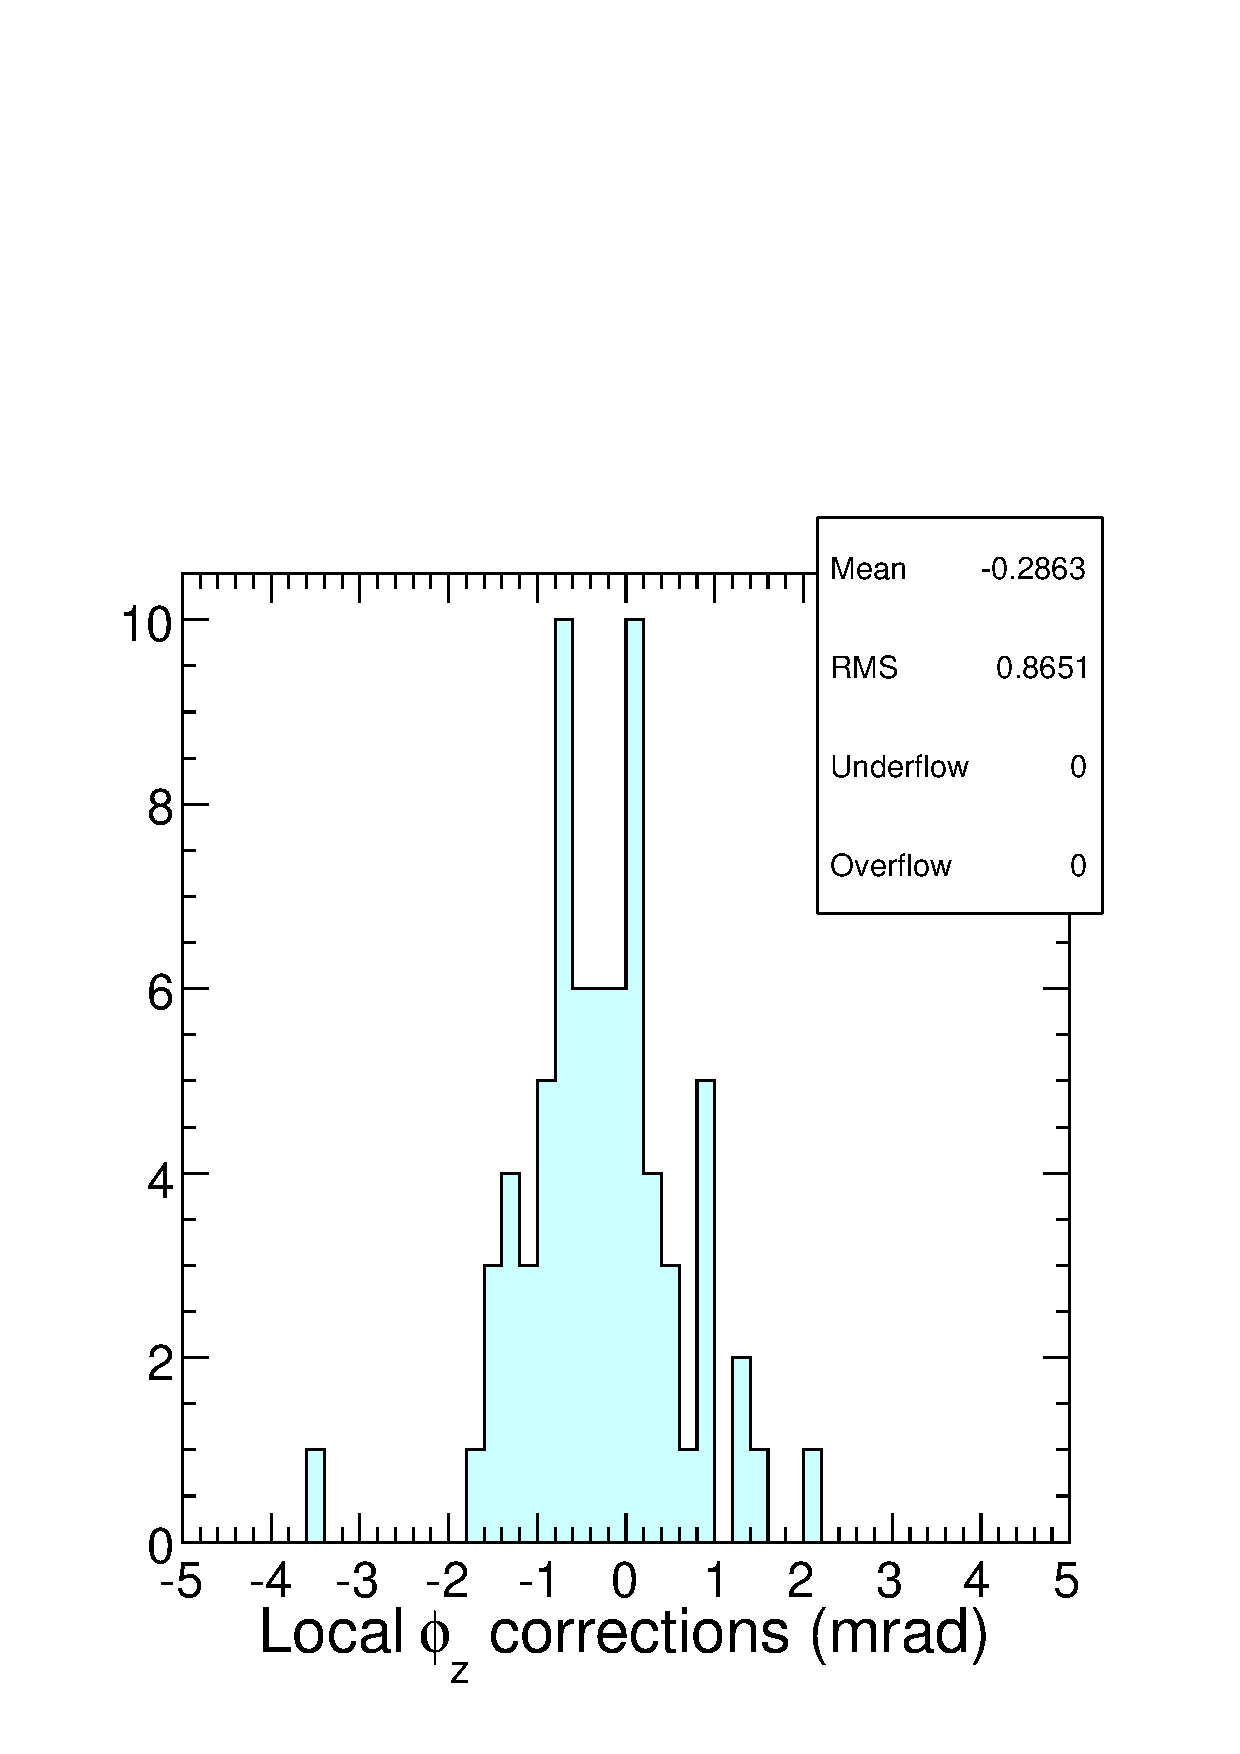
\includegraphics[width=\linewidth]{corrections_phiz.pdf}
\end{columns}

\vfill
\begin{itemize}
\item 5--10~mm changes in $r\phi$ positions, but they don't correspond to an overall rotation of the wheels

\item A scan of residuals differences plots suggests that remaining misalignment is on the order of 1--2~mm

\item Also important: apparent stretching of DT chambers (see epilogue)
\end{itemize}
\end{frame}

%% \section*{First section}
%% \begin{frame}
%% \begin{center}
%% \Huge \textcolor{blue}{First section}
%% \end{center}
%% \end{frame}

\begin{frame}
\frametitle{Conclusions}
\begin{itemize}\setlength{\itemsep}{0.2 cm}
\item Proposal for CRAFT:

\vspace{0.1 cm}
upload these constants with \mbox{optional minor updates:\hspace{-1 cm}}
\begin{itemize}
\item we could drop local $y$ corrections at this stage
\item if so, we could take advantage of the tracker TEC (bias was in $z$ direction, not $r\phi$)
\item lower threshold for chamber alignment (fewer unaligned chambers, more consistent system)
\end{itemize}

\item Constants-generation takes about 2--3~hours, validation suite takes 10--20~minutes on an empty CAF
\begin{itemize}
\item available on demand
\end{itemize}
\end{itemize}

\vfill

\label{numpages}
\end{frame}

\begin{frame}
\begin{center}
\Huge \textcolor{blue}{Epilogue: DT chamber stretching}
\end{center}
\end{frame}

\begin{frame}
\frametitle{The clue (\only<1>{1}\only<2>{2}\only<3>{3}/3)}

\only<1>{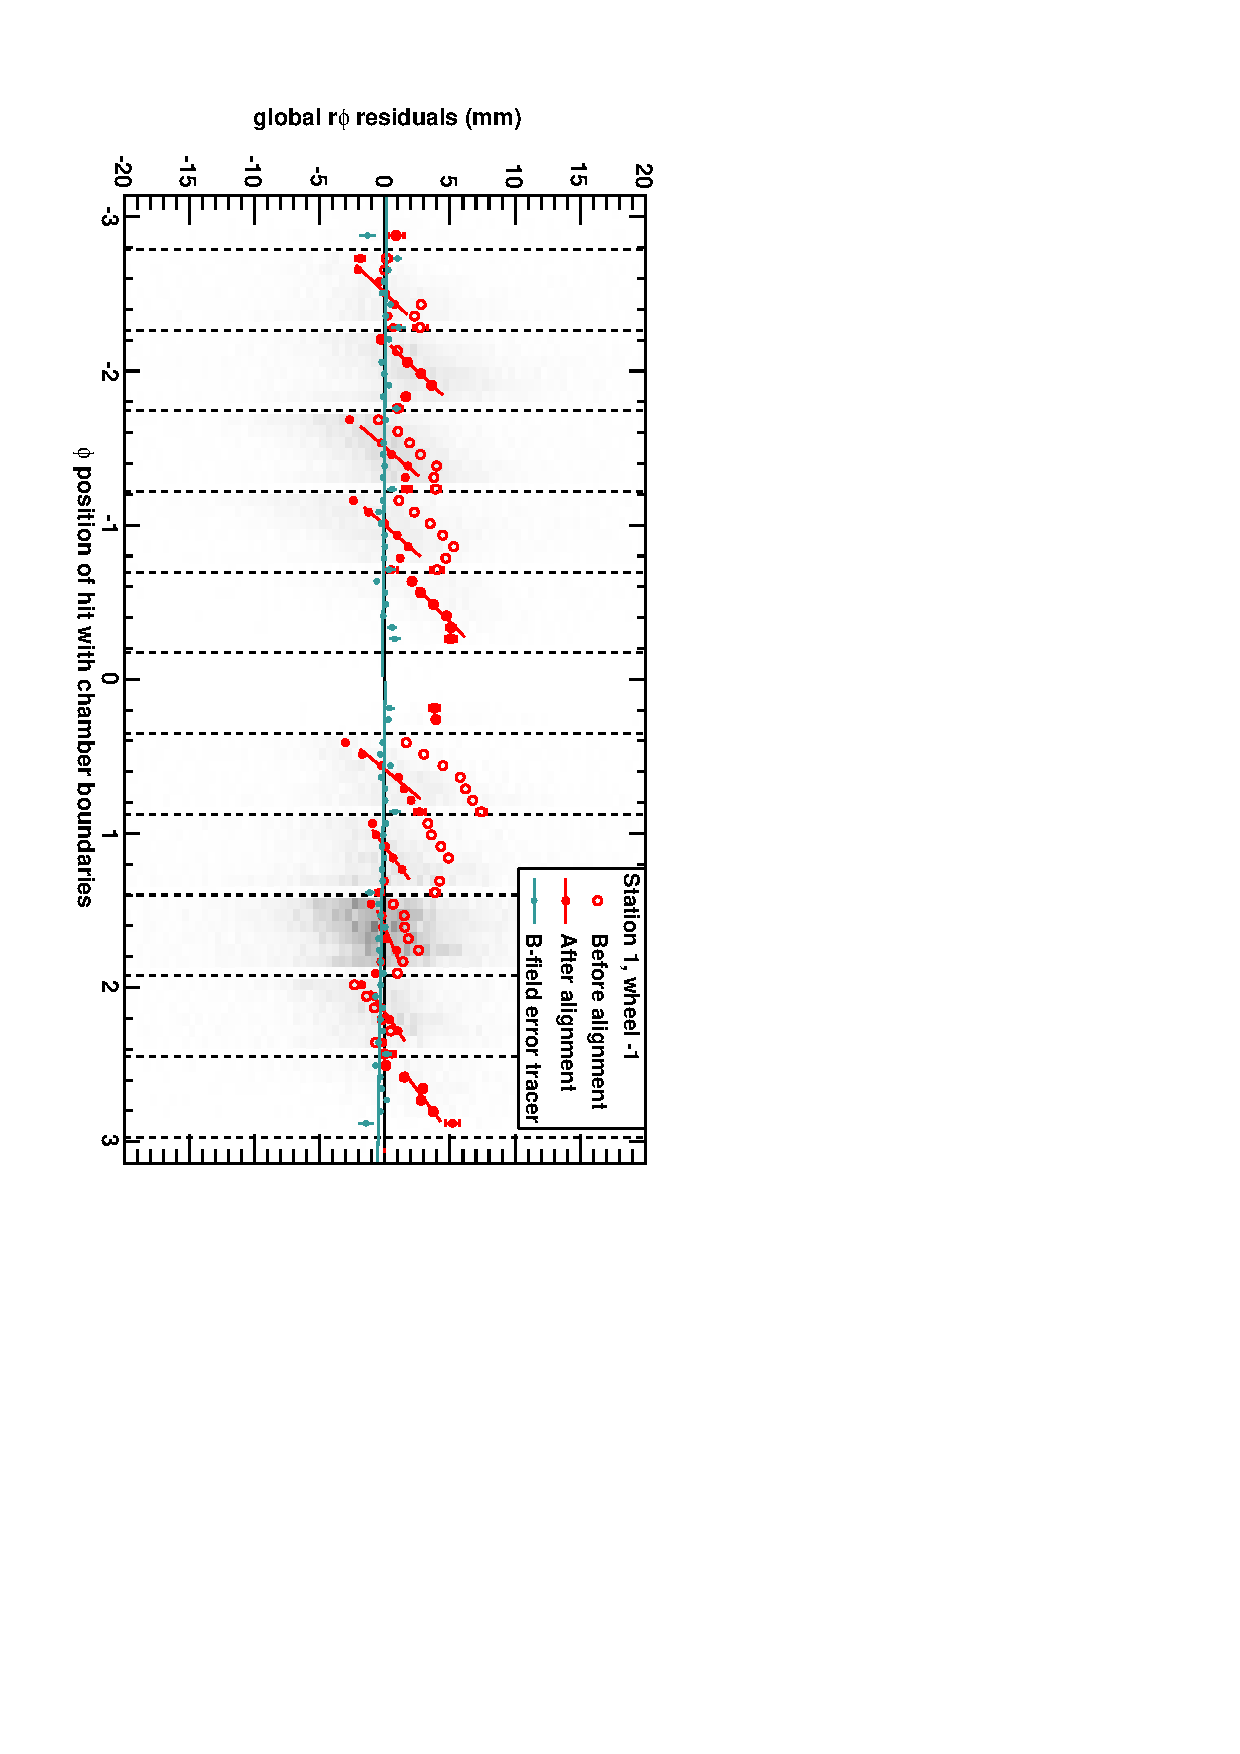
\includegraphics[height=\linewidth, angle=90]{DTrphiVsPhi_st1_whB.pdf}}
\only<2>{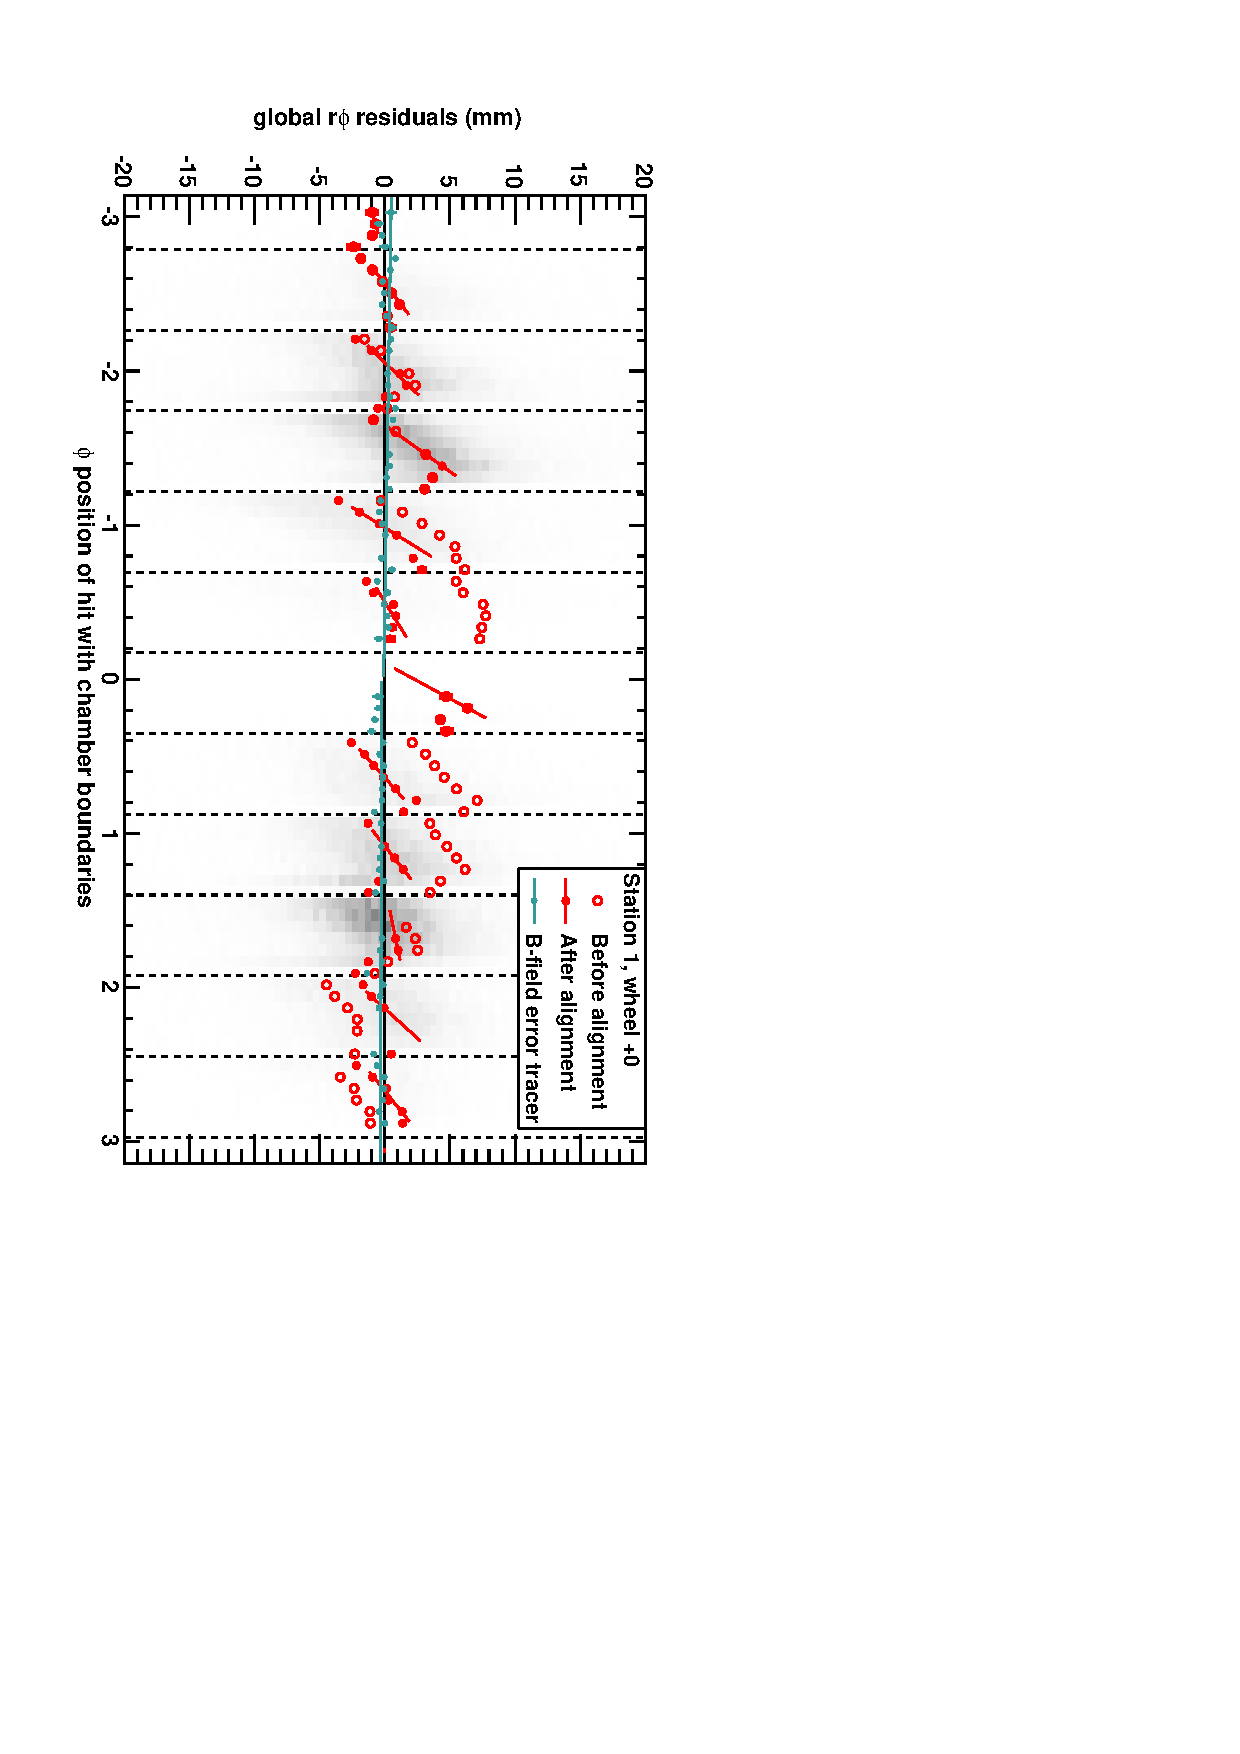
\includegraphics[height=\linewidth, angle=90]{DTrphiVsPhi_st1_whC.pdf}}
\only<3>{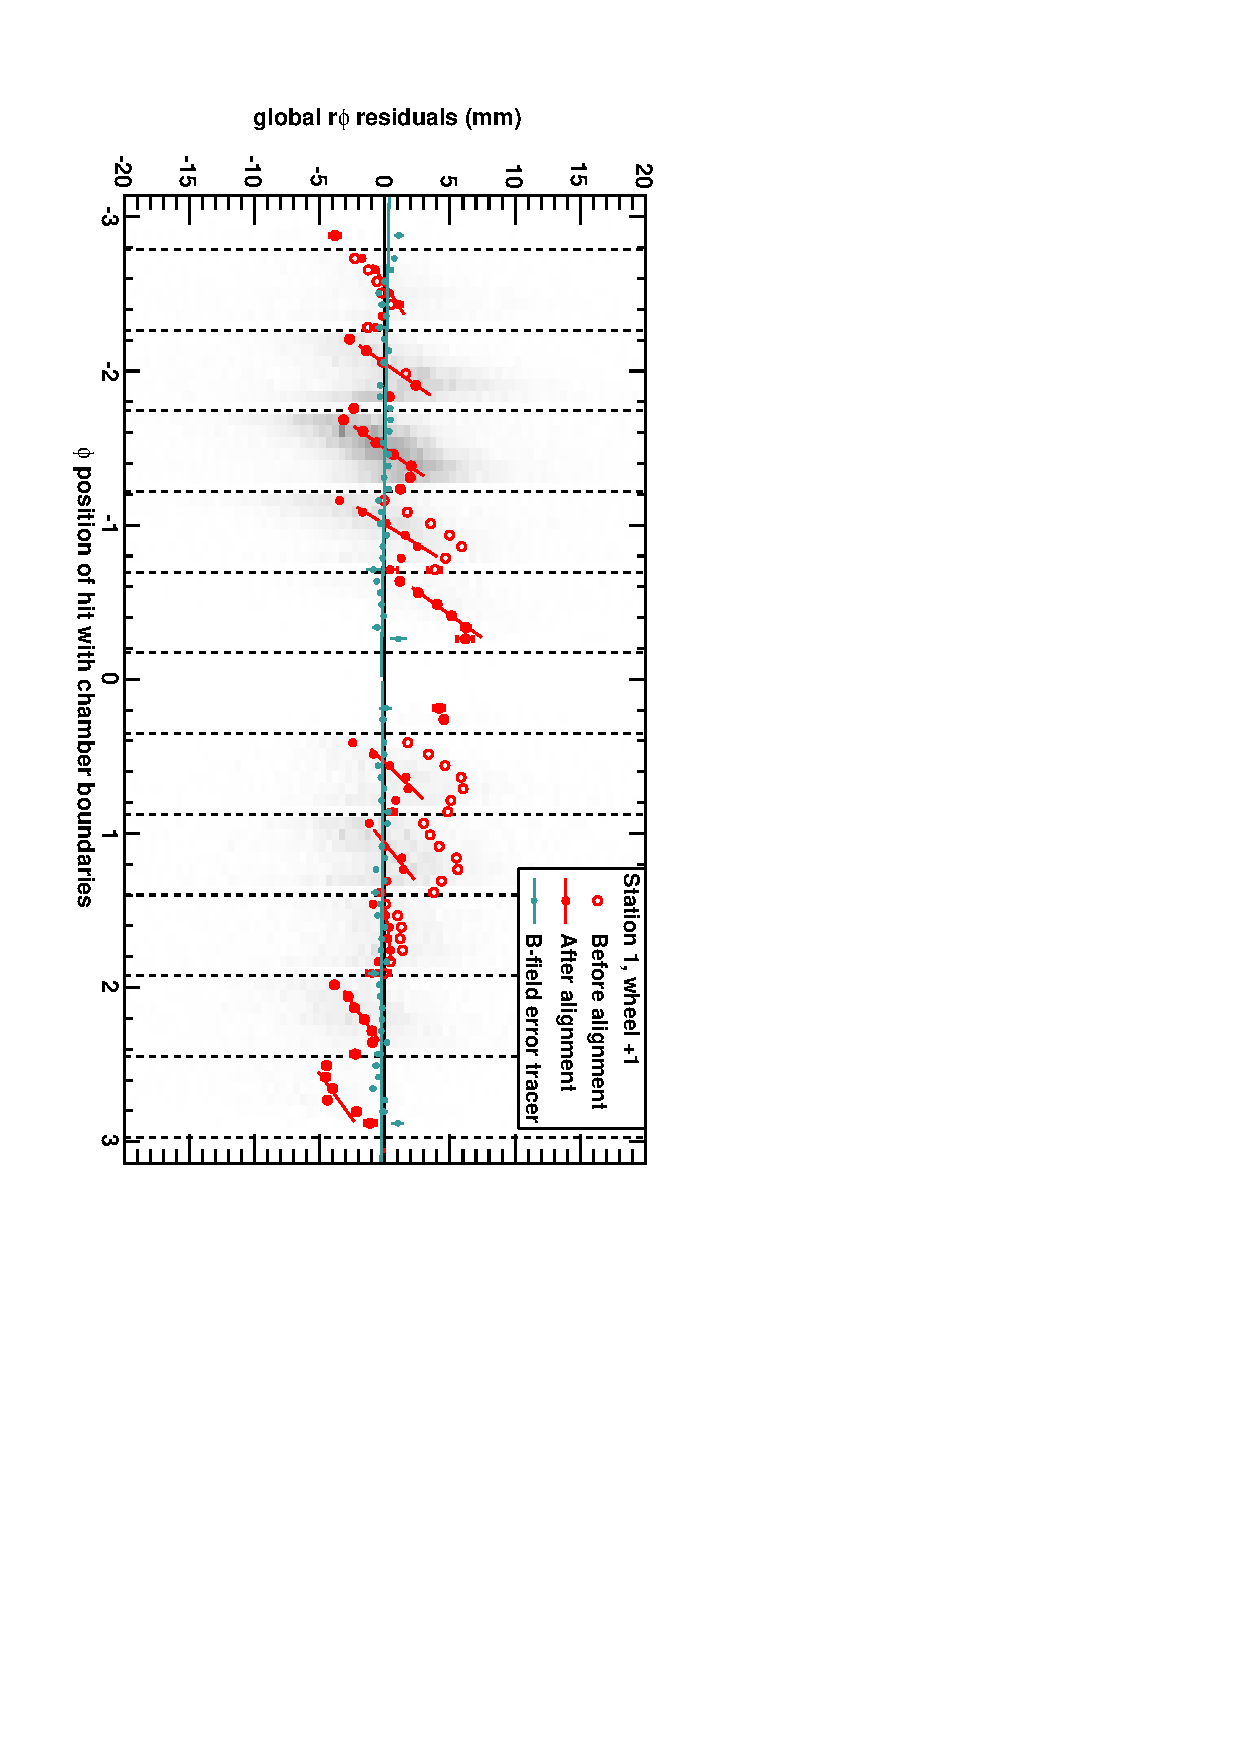
\includegraphics[height=\linewidth, angle=90]{DTrphiVsPhi_st1_whD.pdf}}

\vspace{-0.5 cm}
\only<1>{\begin{itemize}
\item Linear trends in unbiased $r\phi$ residual vs.\ $\phi$ inside each chamber
\item Unaffected by local $x$ alignment (as expected)
\item Curious thing: they all seem to have the same slope
\end{itemize}}
\only<2>{\begin{itemize}
\item What if it's a linear bias in the distribution from the track source, partly absorbed by the alignment?
\begin{itemize}
\item impossible: $\phi$ must have periodic boundary conditions
\item if we realigned chambers to make a continuous line, it could not match at $\pm\pi$ (it would fail a ``closure condition'')
\end{itemize}
\end{itemize}}
\only<3>{\begin{itemize}
\item So it's a real effect related to the chambers, not the track source
\begin{itemize}
\item not fixing it would smear chamber resolution by 5~mm!
\end{itemize}
\item What rigid body misalignments can cause it?
\begin{itemize}
\item $\phi_y$ (rotation around axis parallel to the beamline)
\item $\Delta R$ (radial displacements)
\end{itemize}
\end{itemize}}
%% \hspace{-0.83 cm} \textcolor{darkblue}{\Large Outline2}
\end{frame}

\begin{frame}
\frametitle{The $\phi_y$ possibility}

\begin{columns}
\column{0.5\linewidth}
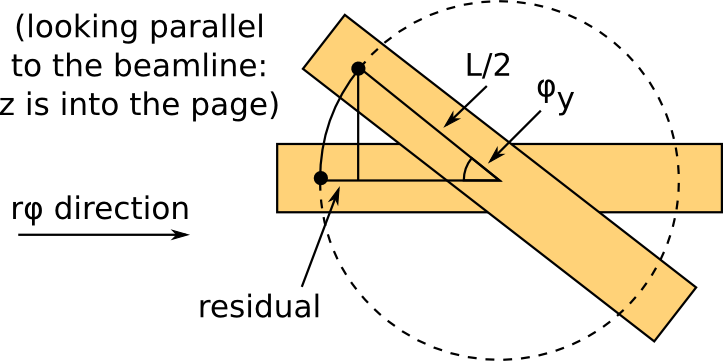
\includegraphics[width=\linewidth]{phiy_explanation.png}

\column{0.5\linewidth}
\begin{itemize}
\item $\phi_y$ rotation can make a chamber appear narrower
\item but it's a second-order effect:
\end{itemize}

\vspace{-0.75 cm}
\begin{eqnarray*}
\mbox{residual} &=& (L/2) \left(1 - \cos\phi_y\right) \\
\phi_y &\approx& \mbox{70~mrad}
\end{eqnarray*}
\end{columns}

\vfill
\begin{itemize}
\item Could {\it all} the chambers be independently misaligned by about 70~mrad?
\item Same effect observed in IDEAL and CRAFT\_ALL\_V4 constants: it
  would have to be a physical misalignment of real chambers
\item I think we can safely say that this is not what's happening
\begin{itemize}
\item the magnitude is too big, and
\item the pattern is too regular
\end{itemize}
\end{itemize}
\end{frame}

\begin{frame}
\frametitle{The $\Delta R$ possibility}

\begin{columns}
\column{0.7\linewidth}
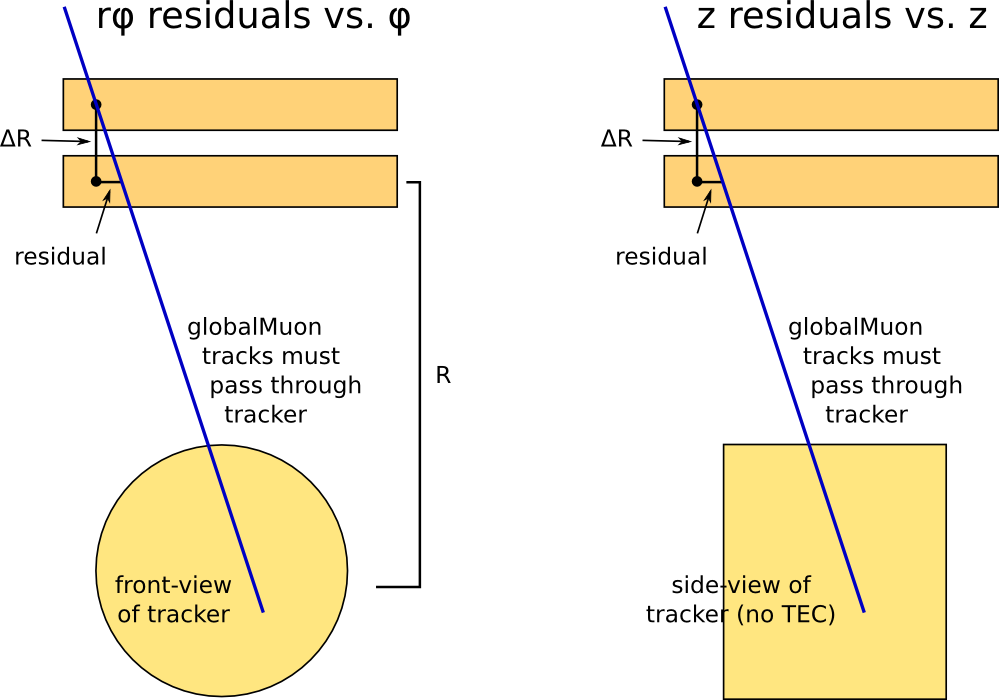
\includegraphics[width=\linewidth]{z_explanation.png}

\column{0.3\linewidth}
\begin{itemize}
\item A track sample constrained to pass through the tracker can introduce effects of this sort

\vspace{0.2 cm}
\mbox{\hspace{-1 cm}$\displaystyle \Delta R = \frac{R}{(L/2)} \left(\mbox{residual}\right)$\hspace{-1 cm}}

\vspace{0.1 cm}
\item But it has to appear in both types of residuals
\end{itemize}
\end{columns}
\end{frame}

\begin{frame}
\frametitle{Trial $\Delta R$ alignment (1/2)}

\begin{itemize}
\item To see if this is plausible, I expanded the radius of all DT stations by 15~mm in a private test
\begin{itemize}
\item seems to cancel the $r\phi$ residual vs.\ $\phi$ trend in the $-\pi < \phi < 0$ range, but overshoot slightly in the $0 < \phi < +\pi$ range
\end{itemize}
\end{itemize}

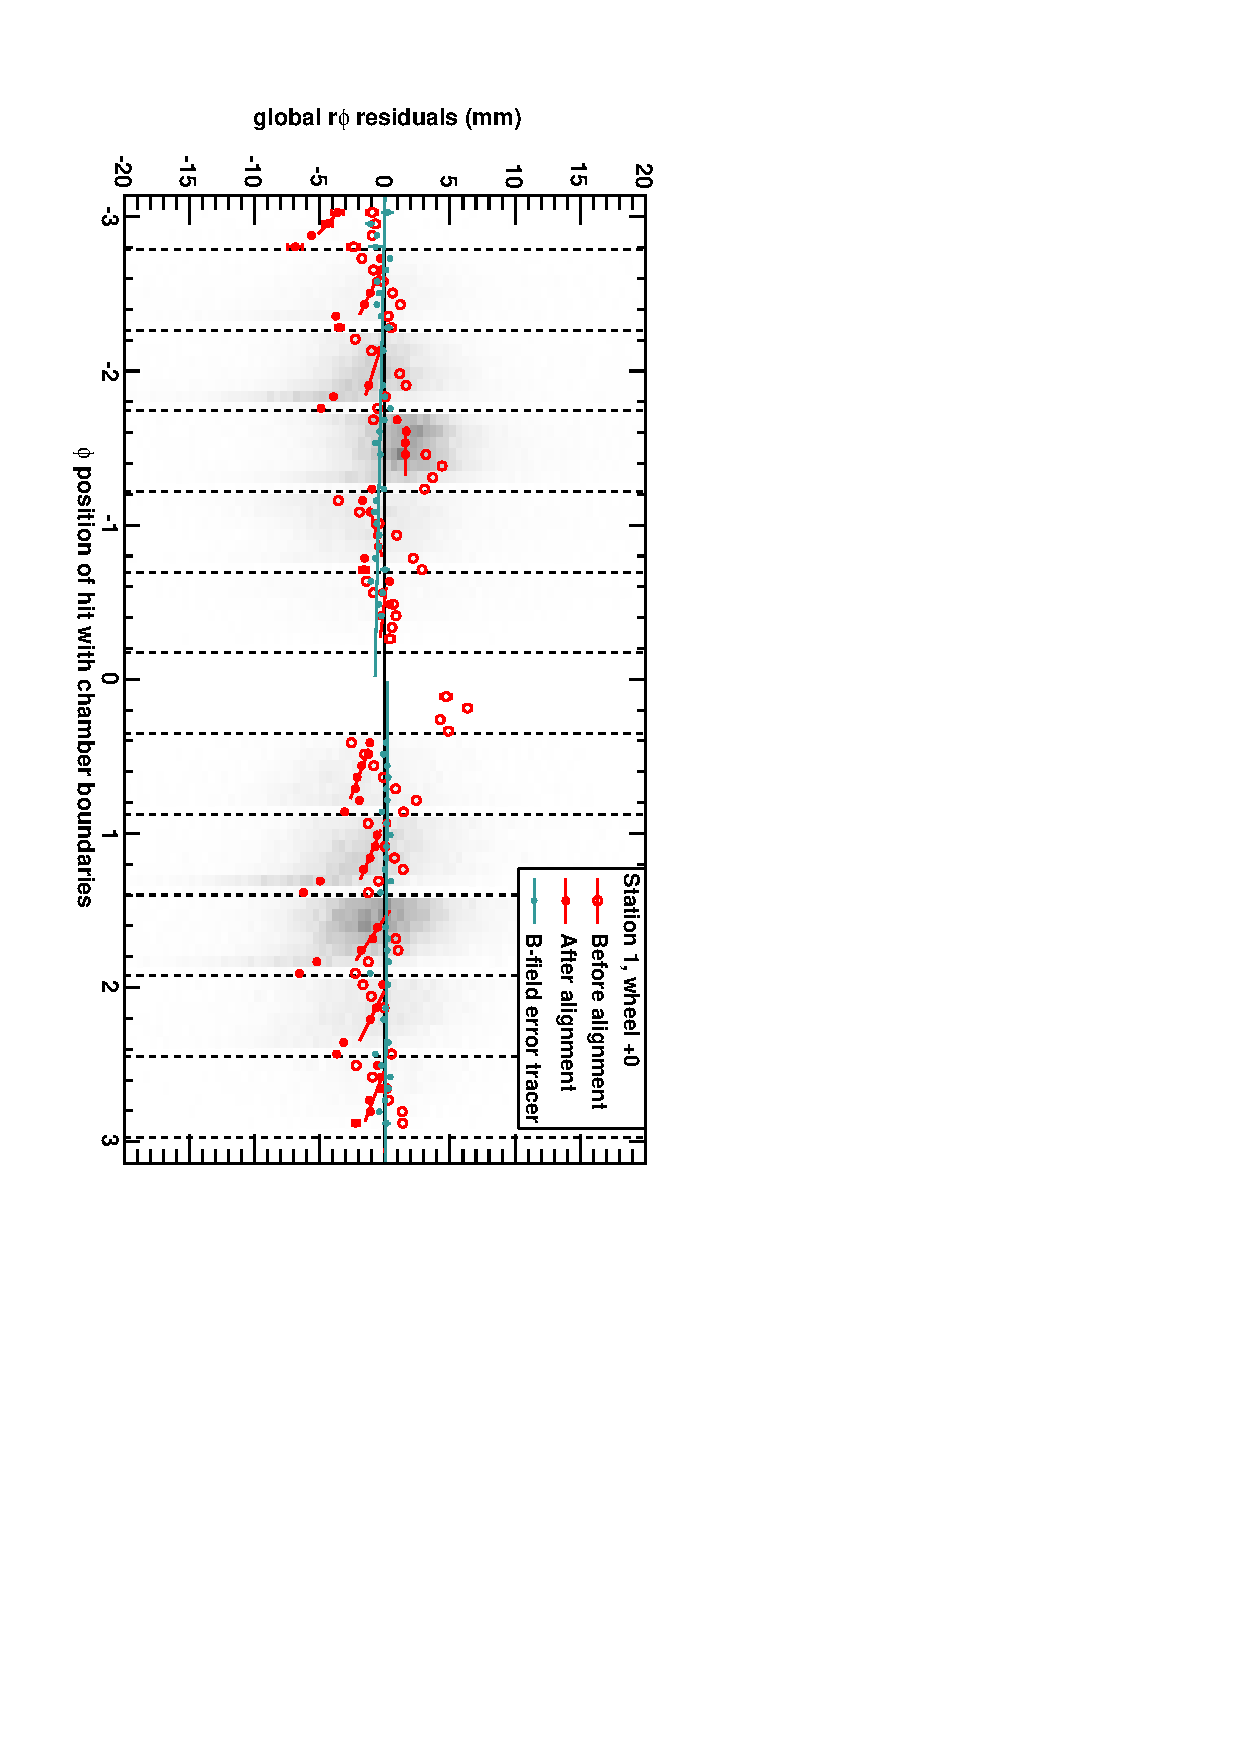
\includegraphics[height=\linewidth, angle=90]{DTrphiVsPhi_st1_whC_out15mm.pdf}
\end{frame}

\begin{frame}
\frametitle{Trial $\Delta R$ alignment (2/2)}

\begin{itemize}
\item However, look what happens to the $z$ residual vs.\ $z$: clearly both types of residuals can't be satisfied!
\item The open circles are the case of no $\Delta R$ shift
\end{itemize}

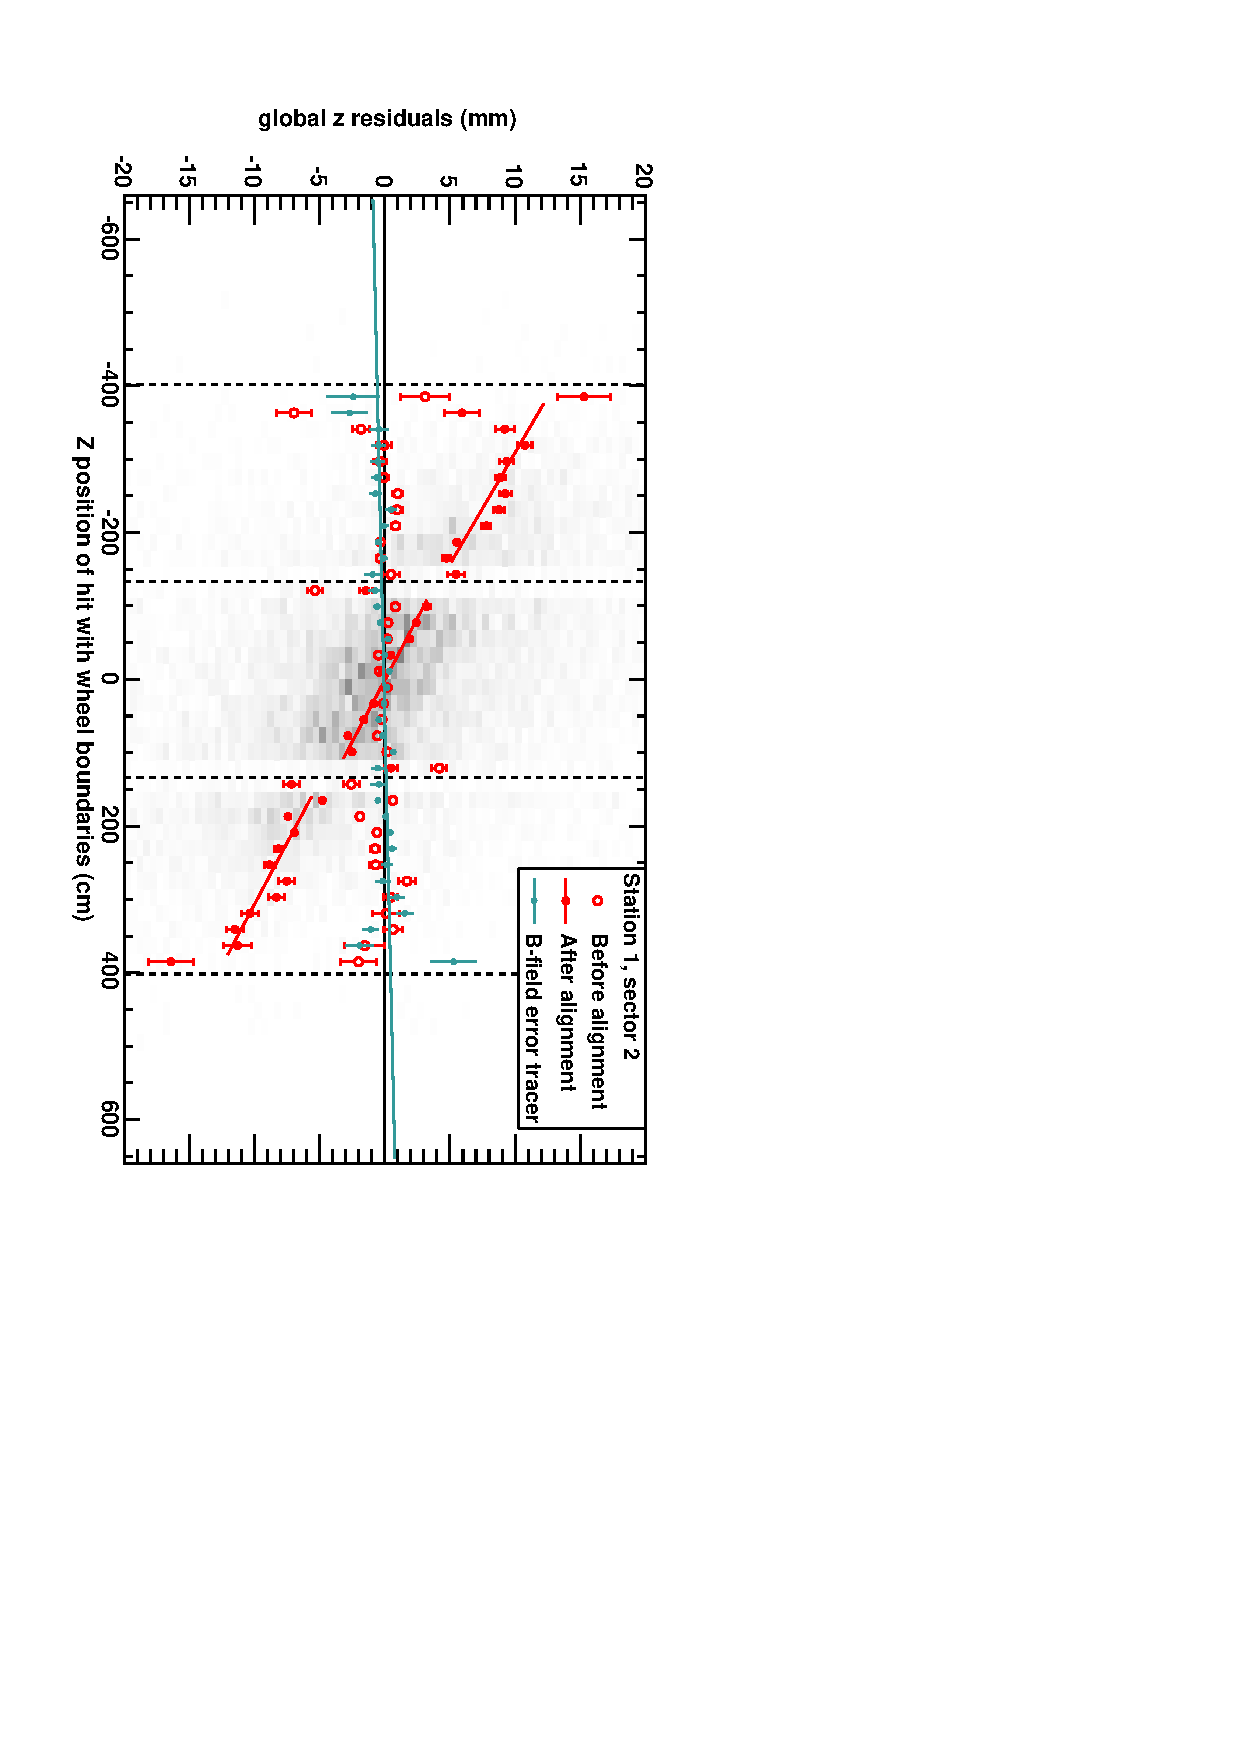
\includegraphics[height=\linewidth, angle=90]{DTzVsZ_st1_sr02_out15mm.pdf}
\end{frame}

\begin{frame}
\frametitle{So, what could it be?}

\begin{itemize}
\item Process of elimination for all rigid body degrees of freedom

\begin{itemize}
\item \sout{$\phi_y$: implausible}
\item \sout{$\Delta R$ (a local $z$ translation): can't reconcile both $r\phi$ and $z$ residuals}
\item local $x$, $y$ translations: can't introduce any linear trends in residuals, only offsets
\item $\phi_z$ rotation: introduces a linear trend in $r\phi$
  residuals vs.\ $z$ and $z$ residuals vs.\ $\phi$, but not what we're
  looking for
\item $\phi_x$ rotation: also would have to be implausibly large, and only affects $z$ residuals (the opposite of what we're looking for)
\end{itemize}

\item Non-rigid degree of freedom \hfill 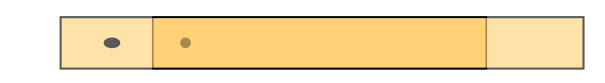
\includegraphics[width=0.35\linewidth]{stretch_explanation.png}

\begin{itemize}
\item {\it some kind} of stretching would easily explain it
\item an error in the geometry description, duplicated by CMSSW, would
  account for its regularity (with outliers due to small individual
  $\Delta R$ misalignments)
\end{itemize}
\end{itemize}
\end{frame}

\begin{frame}
\frametitle{Analogy with CSC case}
\begin{itemize}
\item Last year, a similar track-based technique uncovered a 0.8~mm error in CSC widths
\item For the same reasons, chamber stretching was degenerate with increasing the distance from the beamline
\item Degeneracy was resolved with photogrammetry of alignment pins
\begin{itemize}
\item track-based procedure reproduced $r\phi$ positions of alignment pins with 270~$\mu$m accuracy
\item $R$ positions of pins were therefore directly comparable, and constrained distance from the beamline
\end{itemize}
\item CSC geometry experts investigated and quickly found a 10~$\mu$m strip pitch
  angle error, which, compounded over 80~strips, changed the width by
  0.8~mm, explaining the observation with tracks
\item DTs have an advantage over CSCs in that they precisely measure
  $z$ residuals in addition to $r\phi$ residuals, so we can already
  break degeneracy between $\Delta R$ and stretching
\item In the CSC case, we predicted the magnitude but made a mistake in guessing
  the sign: we'd follow up on any effect of this magnitude
\end{itemize}
\end{frame}

\begin{frame}
\frametitle{Conclusions: what to do?}
\begin{itemize}\setlength{\itemsep}{0.2 cm}
\item I would like to ask DT geometry experts to look for a chamber
  description error on the order of 5~mm across the local $x$
  dimension

\item We have shown that it is a real chamber-level effect and ruled
  out the possibility of it being caused by any rigid chamber misalignment

\item ``Stretching/squashing'' can be interpreted loosely
\begin{itemize}
\item only distortions which affect active elements matter
\item a bulging layer can look narrow (though that's a second-order effect, like $\phi_y$)
\item a $\phi_y$ $\sim$ 70~mrad rotation built into the chamber?
\item a $\Delta R$ misalignment for superlayers 1 and 3 and not superlayer 2 could explain the incompatibility of $r\phi$ and $z$ residuals
\item it's hard to imagine timing effects playing a role, since left- and right-hand sides of each wire would be affected oppositely
\item \ldots
\end{itemize}

\item Since it's causing $\pm 2.5$~mm unbiased residuals errors at the ends of
  the chambers, it's as important for resolution as alignment

\end{itemize}
\end{frame}

\end{document}
